%%%%%%%%%%%%%%%%%%%%%%%%%%%%%%%%%%%%%%%%%%%%%%%%%%%%%%%%%%%%%%%%
\begin{frame}[fragile]\frametitle{}
\begin{center}
{\Large ZenYoga Chapters}


{\tiny (Based on ``Zen Yoga'' by P J Saher and YouTube Channels by Abhishen, Ashish Shukla)}
\end{center}
\end{frame}

%%%%%%%%%%%%%%%%%%%%%%%%%%%%%%%%%%%%%%%%%%%%%%%%%%%%%%%%%%%%%%%%
\begin{frame}[fragile]\frametitle{}
\begin{center}
{\Large Part I}
\end{center}
\end{frame}

%%%%%%%%%%%%%%%%%%%%%%%%%%%%%%%%%%%%%%%%%%%%%%%%%%%%%%%%%%%%%%%%
\begin{frame}[fragile]\frametitle{}
\begin{center}
{\Large Chapter 1: Mind and Thinking}
\end{center}
\end{frame}

%%%%%%%%%%%%%%%%%%%%%%%%%%%%%%%%%%%%%%%%%%%%%%%%%%%%%%%%%%%%%%%%
\begin{frame}[fragile]\frametitle{Introduction}

\begin{itemize}
    \item The chapter discusses the mind, its thinking process, and how both interact.
    \item How thoughts influence the mind and how the mind gets distracted.
    \item Examples are provided to show how our thoughts drift and how we lose track of the original subject.
\end{itemize}

\end{frame}


%%%%%%%%%%%%%%%%%%%%%%%%%%%%%%%%%%%%%%%%%%%%%%%%%%%%%%%%%%%%%%%%
\begin{frame}[fragile]\frametitle{Types of Drifting Thoughts}

\begin{itemize}
    \item Drifting thoughts can be classified into:
    \begin{itemize}
        \item Controllable drifts
        \item Uncontrollable drifts
        \item Unrecognized drifts
    \end{itemize}
    \item Controllable drifts: When we realize the mind has drifted and we bring it back to the original subject.
    \item Uncontrollable drifts: When we completely forget the original subject and cannot recall how we got there.
\end{itemize}

\end{frame}

%%%%%%%%%%%%%%%%%%%%%%%%%%%%%%%%%%%%%%%%%%%%%%%%%%%%%%%%%%%%%%%%
\begin{frame}[fragile]\frametitle{Drifting Thoughts: Examples}

\begin{itemize}
    \item Example of controllable drift: 
        \begin{itemize}
            \item We start thinking about one subject, but our mind wanders. 
            \item Realizing the drift, we bring ourselves back to the original thought.
        \end{itemize}
    \item Example of uncontrollable drift: 
        \begin{itemize}
            \item The mind jumps from one thought to another, and eventually, we forget what we were originally thinking about.
        \end{itemize}
\end{itemize}

\end{frame}

%%%%%%%%%%%%%%%%%%%%%%%%%%%%%%%%%%%%%%%%%%%%%%%%%%%%%%%%%%%%%%%%
\begin{frame}[fragile]\frametitle{Impact of Thoughts on Actions}

\begin{itemize}
    \item Our thoughts are directly connected to our actions.
    \item Understanding the thinking process helps shape our life.
    \item If we don’t control our thoughts, we may end up in a difficult mental state.
    \item We are responsible for our thoughts, and in turn, our actions and life direction.
\end{itemize}

\end{frame}

%%%%%%%%%%%%%%%%%%%%%%%%%%%%%%%%%%%%%%%%%%%%%%%%%%%%%%%%%%%%%%%%
\begin{frame}[fragile]\frametitle{Mind and Thought Control}

\begin{itemize}
    \item If we cannot control our thoughts, it can lead to an uncontrolled mental state, or "mind drift."
    \item By understanding the nature of mind and thoughts, we can learn to control and redirect them.
    \item Meditation can help in recognizing the thought processes and bring the mind back to focus.
\end{itemize}

\end{frame}

%%%%%%%%%%%%%%%%%%%%%%%%%%%%%%%%%%%%%%%%%%%%%%%%%%%%%%%%%%%%%%%%
\begin{frame}[fragile]\frametitle{Meditation and Mind Control}

\begin{itemize}
    \item Meditation involves observing the drifting thoughts without attachment.
    \item It helps in understanding which part of the mind is active and dominant.
    \item Achieving a focused, clear state of mind is the goal of meditation.
\end{itemize}

\end{frame}

%%%%%%%%%%%%%%%%%%%%%%%%%%%%%%%%%%%%%%%%%%%%%%%%%%%%%%%%%%%%%%%%
\begin{frame}[fragile]
\frametitle{Drift Order}
\begin{itemize}
\item Drifts happen in the section of mind that deals with pictures, day-dreams.
\item Typically the come in this order:
\begin{itemize}
\item Sexual
\item Anger
\item Ego
\item Greed
\item Jealousy
\item Arrogance
\item Ignorance
\item Courage
\item Doubt
\item Day dreaming
\end{itemize}
\end{itemize}
\end{frame}


%%%%%%%%%%%%%%%%%%%%%%%%%%%%%%%%%%%%%%%%%%%%%%%%%%%%%%%%%%%%%%%%
\begin{frame}[fragile]\frametitle{Summary}

\begin{itemize}
	\item Drift: Change in thoughts away from the main subject.
	\item Types:
		\begin{itemize}
			\item Un-controllable: Unaware of it, can not recollect
			\item Controllable: Can detect and come back to the main subject.
		\end{itemize}
	\item Mind, if not trained, can not channelize drifts.
	\item This drift is not property of the whole mind but one section within it.
	\item So, learn to separate sections of mind and understand the functionality.
    \item Understanding mind and thought drifts is essential for self-awareness and personal growth.
    \item Thoughts lead to actions, and actions shape our lives.
    \item Meditation and mindfulness can help control the mind and direct it towards constructive actions.
    \item Mastery over thoughts leads to a harmonious and controlled life.
\end{itemize}

\end{frame}

%%%%%%%%%%%%%%%%%%%%%%%%%%%%%%%%%%%%%%%%%%%%%%%%%%%%%%%%%%%%%%%%
\begin{frame}[fragile]\frametitle{}
\begin{center}
{\Large Chapter 2: Drifts of the Mind and What they convey?}
\end{center}
\end{frame}


%%%%%%%%%%%%%%%%%%%%%%%%%%%%%%%%%%%%%%%%%%%%%%%%%%%%%%%%%%%%%%%%
\begin{frame}[fragile]\frametitle{Introduction}
  \begin{itemize}
    \item This chapter focuses on three main concepts in Zenyoga: Simple Consciousness, Self-Consciousness, and Cosmic Consciousness.
    \item Simple Consciousness: Present in all living beings, including animals and humans.
    \item Self-Consciousness: Exclusive to humans, which helps us observe and control our mind's state.
    \item Cosmic Consciousness: A higher state of awareness that transcends individual identity.
  \end{itemize}
\end{frame}

%%%%%%%%%%%%%%%%%%%%%%%%%%%%%%%%%%%%%%%%%%%%%%%%%%%%%%%%%%%%%%%%
\begin{frame}[fragile]\frametitle{Simple Consciousness}
  \begin{itemize}
    \item Simple consciousness is a state present in all living beings.
    \item It allows us to be aware of our surroundings and react accordingly.
    \item This awareness is crucial for survival and adaptation to the environment.
    \item Animals also experience simple consciousness but lack the ability to reflect on their mental states.
  \end{itemize}
\end{frame}

%%%%%%%%%%%%%%%%%%%%%%%%%%%%%%%%%%%%%%%%%%%%%%%%%%%%%%%%%%%%%%%%
\begin{frame}[fragile]\frametitle{Self-Consciousness}
  \begin{itemize}
    \item Self-consciousness is unique to humans, allowing us to reflect on and control our mental states.
    \item Humans can observe their mood swings and emotions throughout the day.
    \item This ability to reflect and evolve one's mind is a key aspect of human nature.
    \item Unlike animals, humans can identify their identity and separate it from the environment.
  \end{itemize}
\end{frame}

%%%%%%%%%%%%%%%%%%%%%%%%%%%%%%%%%%%%%%%%%%%%%%%%%%%%%%%%%%%%%%%%
\begin{frame}[fragile]\frametitle{Challenges in Self-Consciousness}
  \begin{itemize}
    \item While humans have the potential for self-awareness, it is often difficult to concentrate and meditate.
    \item Our comfort zone and habits prevent us from evolving our minds effectively.
    \item The difficulty lies in sustaining concentration and overcoming habitual patterns.
  \end{itemize}
\end{frame}

%%%%%%%%%%%%%%%%%%%%%%%%%%%%%%%%%%%%%%%%%%%%%%%%%%%%%%%%%%%%%%%%
\begin{frame}[fragile]\frametitle{Cosmic Consciousness}
  \begin{itemize}
    \item Cosmic consciousness is a higher state of awareness that transcends individual identity.
    \item It is a state where one feels a deep connection with the universe.
    \item Achieving this state requires overcoming the distractions of the mind and focusing on a higher subject.
    \item It is a state that few have achieved due to the complexity of human tendencies.
  \end{itemize}
\end{frame}

%%%%%%%%%%%%%%%%%%%%%%%%%%%%%%%%%%%%%%%%%%%%%%%%%%%%%%%%%%%%%%%%
\begin{frame}[fragile]\frametitle{The Story of Narada and Krishna}
  \begin{itemize}
    \item Narada Muni asks Lord Krishna why humans remain trapped in the illusion of the physical world.
    \item Krishna explains that humans have the potential to achieve enlightenment but are distracted by the mind’s tendencies.
    \item Narada Muni forgets his mission to bring water for Krishna after being distracted by a woman at the river.
    \item The woman reveals herself to be Krishna, demonstrating how even enlightened beings can be distracted by worldly matters.
  \end{itemize}
\end{frame}



%%%%%%%%%%%%%%%%%%%%%%%%%%%%%%%%%%%%%%%%%%%%%%%%%%%%%%%%%%%%%%%%
\begin{frame}[fragile]\frametitle{Exercise}
\begin{itemize}
\item Put aside 15-30 minutes in a day to watch the drifts and note them down.
\item Take one thought as the main subject.
\item Let the mind drift.
\item Classify and note the drift.
\item Never try to make your mind ``blank''.
\item Analyze over 3 months, the persistent patterns.
\item After 15 days of consistent practice, you will start recognizing which mental centers dominate your mind.
\item Over time, this awareness will help you overcome mental distractions and develop a deeper connection with the 
\end{itemize}
\end{frame}




%%%%%%%%%%%%%%%%%%%%%%%%%%%%%%%%%%%%%%%%%%%%%%%%%%%%%%%%%%%%%%%%
\begin{frame}[fragile]\frametitle{Summary}
Forms of Consciousness:
\begin{itemize}
\item Simple: like animals, awareness of body. Needed for daily survival.
\item Self: Aware of mental states, sense of self, thoughts.
\item Cosmic: Higher state. Not achieved by logic, reasoning, etc but by stronger awareness.
\item No one has shown practical steps to go from Self to Cosmic consciousness.
\item Even if we get to know the steps, they are difficult to follow. Old patterns are hard to break away from.
\item The journey from simple consciousness to cosmic consciousness is challenging but achievable with dedication.
\item Regular practice, patience, and awareness are key to evolving the mind and reaching higher states of consciousness.
\item Zenyoga provides tools to understand and transcend the mind's limitations, leading to enlightenment.
\end{itemize}


\end{frame}


%%%%%%%%%%%%%%%%%%%%%%%%%%%%%%%%%%%%%%%%%%%%%%%%%%%%%%%%%%%%%%%%
\begin{frame}[fragile]\frametitle{}
\begin{center}
{\Large Chapter 3: What is the Mind of Man}
\end{center}
\end{frame}

%%%%%%%%%%%%%%%%%%%%%%%%%%%%%%%%%%%%%%%%%%%%%%%%%%%%%%%%%%%%%%%%
\begin{frame}[fragile]\frametitle{Introduction to Mind and Brain}
\begin{itemize}
    \item \textbf{Mind vs. Brain:} Saher explains that the mind is not equivalent to the physical brain.
    \item The \textbf{mind} is an accumulation of thoughts, while the \textbf{brain} processes these thoughts through sensory inputs.
    \item The brain uses sensory inputs (five senses) to capture, process, and decode external impulses, leading to personal interpretations.
\end{itemize}
\end{frame}

%%%%%%%%%%%%%%%%%%%%%%%%%%%%%%%%%%%%%%%%%%%%%%%%%%%%%%%%%%%%%%%%
\begin{frame}[fragile]\frametitle{Individual Interpretation and Perception}
\begin{itemize}
    \item Each individual interprets external impulses differently based on personal background, environment, and previous experiences.
    \item \textbf{Unique Interpretations:} No two people perceive an event in the exact same way; similar to how people react differently to the same movie.
    \item The mind remains \textbf{invisible}, as it is a collection of thoughts, making self-observation challenging yet essential.
\end{itemize}
\end{frame}

%%%%%%%%%%%%%%%%%%%%%%%%%%%%%%%%%%%%%%%%%%%%%%%%%%%%%%%%%%%%%%%%
\begin{frame}[fragile]\frametitle{Self-Understanding and Observation}
\begin{itemize}
    \item \textbf{Self-Observation:} Observing and understanding one’s thoughts is necessary to understand one's mind.
    \item Modern individuals often lack the time or willingness to introspect, limiting their understanding of themselves and others.
    \item Saher emphasizes that \textbf{self-reflection} enables clarity in understanding both oneself and others.
\end{itemize}
\end{frame}

%%%%%%%%%%%%%%%%%%%%%%%%%%%%%%%%%%%%%%%%%%%%%%%%%%%%%%%%%%%%%%%%
\begin{frame}[fragile]\frametitle{Connection with Others’ Minds}
\begin{itemize}
    \item Saher describes three possibilities when minds interact:
    \begin{itemize}
        \item \textbf{Affinity:} Similar thoughts lead to friendship, love, or positive relationships.
        \item \textbf{Repulsion:} Differences in thought can lead to disagreement, negativity, and hostility.
        \item \textbf{Indifference:} Lack of emotional reaction, potentially leading to detachment or even depression.
    \end{itemize}
\end{itemize}
\end{frame}

%%%%%%%%%%%%%%%%%%%%%%%%%%%%%%%%%%%%%%%%%%%%%%%%%%%%%%%%%%%%%%%%
\begin{frame}[fragile]\frametitle{The Nature of Mind and Emotions}

\begin{itemize}
    \item Saher likens the mind to a \textbf{fabric woven from various thoughts}, colored by emotions.
    \item \textbf{Emotions} act as dyes, influencing the overall tone of the mind.
    \item \textbf{Habits and Patterns:} Positive habits strengthen the mind, while emotional quality affects its openness, resilience, and overall character.
\end{itemize}
\end{frame}

%%%%%%%%%%%%%%%%%%%%%%%%%%%%%%%%%%%%%%%%%%%%%%%%%%%%%%%%%%%%%%%%
\begin{frame}[fragile]
\frametitle{Mind as a Cloth}
\begin{itemize}
\item Thoughts are strands
\item Emotions are the colors
\item Repetition or habit strengthens and makes cloth durable.
\item Quality of thoughts correspond to smoothness or roughness of the cloth.
\item Grey matter, attitude, thought process: Shape of the cloth
\item Likes/Dislikes: fashion of the cloth.
\end{itemize}

Constant daily practice can change the properties of the cloth.
\end{frame}

%%%%%%%%%%%%%%%%%%%%%%%%%%%%%%%%%%%%%%%%%%%%%%%%%%%%%%%%%%%%%%%%
\begin{frame}[fragile]\frametitle{The Influence of Thoughts on Personality}

\begin{itemize}
    \item Thoughts accumulate over time, shaping \textbf{personality} and \textbf{character}.
    \item \textbf{Intelligence and Reflection:} Using intelligence helps define character by understanding and refining thoughts.
    \item Individual perception shapes how external impulses are decoded, reinforcing unique mental patterns.
\end{itemize}
\end{frame}

%%%%%%%%%%%%%%%%%%%%%%%%%%%%%%%%%%%%%%%%%%%%%%%%%%%%%%%%%%%%%%%%
\begin{frame}[fragile]\frametitle{Importance of Self-Observation}

\begin{itemize}
    \item Saher encourages \textbf{watching and understanding one's mental patterns}.
    \item Ancient sages could observe both their own and others' thoughts, achieving clarity and wisdom.
    \item Self-awareness helps to evolve one's mind and break free from repetitive thought patterns.
\end{itemize}
\end{frame}

%%%%%%%%%%%%%%%%%%%%%%%%%%%%%%%%%%%%%%%%%%%%%%%%%%%%%%%%%%%%%%%%
\begin{frame}[fragile]\frametitle{Patterns and Automatic Reactions}

\begin{itemize}
    \item Most individuals are \textbf{reactive}, like a tape recorder, responding automatically to stimuli.
    \item External stimuli often govern behavior without conscious understanding.
    \item \textbf{Key to Self-Control:} Observation allows individuals to move from reaction to conscious response.
\end{itemize}
\end{frame}



%%%%%%%%%%%%%%%%%%%%%%%%%%%%%%%%%%%%%%%%%%%%%%%%%%%%%%%%%%%%%%%%
\begin{frame}[fragile]\frametitle{Chapter 3 Summary}
	\begin{itemize}
	\item Brain is a physical entity.
	\item Impulses come from various sensory organs, which perturb the nerves/areas in brain. These are called as `thoughts'.
	\item Collection of thoughts (or the software/platform, in IMHO) is called as `mind'.
	\item Reactions to other minds can be of types:
		\begin{itemize}
			\item Affinity: love
			\item Repulsion: hate
			\item Indifference
		\end{itemize}
	\end{itemize}

\end{frame}




%%%%%%%%%%%%%%%%%%%%%%%%%%%%%%%%%%%%%%%%%%%%%%%%%%%%%%%%%%%%%%%%
\begin{frame}[fragile]\frametitle{}
\begin{center}
{\Large Chapter 4: Do We Think and How?}
\end{center}
\end{frame}


%%%%%%%%%%%%%%%%%%%%%%%%%%%%%%%%%%%%%%%%%%%%%%%%%%%%%%%%%%%%%%%%
\begin{frame}[fragile]\frametitle{Key Concepts of Mind's Impulse Reception and Decoding}
    \begin{itemize}
        \item The mind receives external impulses and decodes them rapidly.
        \item These impulses are registered in specific areas of the brain.
        \item Each person's interpretation and reaction to the same impulse varies.
        \item Influencing factors include: Culture, character, education, circumstances, surroundings, and health.
    \end{itemize}
\end{frame}

%%%%%%%%%%%%%%%%%%%%%%%%%%%%%%%%%%%%%%%%%%%%%%%%%%%%%%%%%%%%%%%%
\begin{frame}[fragile]\frametitle{The Influence of Personal Filters on Thoughts and Actions}
    \begin{itemize}
        \item Impulses registered in the mind start as \textbf{pure mental energy}.
        \item This energy, unaltered initially, becomes modified when interpreted.
        \item Personal characteristics and surroundings color this interpretation.
        \item Thoughts impact personality, mental health, and actions significantly.
    \end{itemize}
\end{frame}

%%%%%%%%%%%%%%%%%%%%%%%%%%%%%%%%%%%%%%%%%%%%%%%%%%%%%%%%%%%%%%%%
\begin{frame}[fragile]\frametitle{Four States of Impulse Processing}
    \begin{itemize}
        \item \textbf{Pure Mental Energy State}: Initial state, unaltered and unprocessed.
        \item \textbf{Thought-Free Symbolic State}: Registered but remains unexpressed in words or images.
        \item \textbf{Mental Imagery State}: Formulated into mental images or daydreaming states.
        \item \textbf{Expressed State in Actions}: Converted into physical actions and expressions.
    \end{itemize}
\end{frame}

%%%%%%%%%%%%%%%%%%%%%%%%%%%%%%%%%%%%%%%%%%%%%%%%%%%%%%%%%%%%%%%%
\begin{frame}[fragile]\frametitle{Understanding Intention vs. Action}
    \begin{itemize}
        \item True actions are judged by intentions, not merely outward expressions.
        \item Actions may not always convey underlying intentions.
        \item Importance of internal purity over external validation.
    \end{itemize}
\end{frame}

%%%%%%%%%%%%%%%%%%%%%%%%%%%%%%%%%%%%%%%%%%%%%%%%%%%%%%%%%%%%%%%%
\begin{frame}[fragile]\frametitle{Insights from Patanjali's Yogasutra}
    \begin{itemize}
        \item Five states of mind affecting pleasure or pain.
        \item Practices like \textbf{Non-attachment} help control mental fluctuations.
        \item \textbf{Constant Effort} (तपस्) is essential to restrain negative modifications.
        \item \textbf{Purification} of mind leads to clarity and cosmic consciousness.
    \end{itemize}
\end{frame}

%%%%%%%%%%%%%%%%%%%%%%%%%%%%%%%%%%%%%%%%%%%%%%%%%%%%%%%%%%%%%%%%
\begin{frame}[fragile]\frametitle{Path to Pure Mind and Cosmic Consciousness}
    \begin{itemize}
        \item Remove filters to perceive the true nature of impulses.
        \item Modifications act as filters, limiting pure awareness.
        \item Pure awareness emerges when filters are removed.
        \item Expanding awareness leads towards cosmic consciousness.
    \end{itemize}
\end{frame}



%%%%%%%%%%%%%%%%%%%%%%%%%%%%%%%%%%%%%%%%%%%%%%%%%%%%%%%%%%%%%%%%
\begin{frame}[fragile]\frametitle{Chapter 4 Summary}
	\begin{itemize}
	\item Incoming impulses are decoded in brain as Pure Mind Energy, which are divided into:
		\begin{itemize}
			\item Held: thoughts suppressed
			\item Words: expressed as words or mental pictures, day dreaming.
			\item Actions: Something is done by them, movements.
		\end{itemize}
	\item As per Patanjali पतंजली , there are 5 states (`vrutti' वृत्ती ) of mind (`chitta' चित्त ):
		\begin{itemize}
			\item Correct Knowledge
			\item Incorrect Knowledge
			\item Fancy
			\item Passivity (sleep)
			\item Memory
		\end{itemize}
	\item Mind can be controlled (``chitta vrutti nirodh:'' चित्त वृत्ती निरोध ) by efforts, detachment.
	\item Peace of mind can be brought by regulation of ``prana'' प्राण (breath).
	\item Mental purification and clarity are keys to true perception.
	\item Detaching from modifications allows pure awareness to arise.
	\item Regular practice leads to cosmic consciousness and expansive awareness.	
	\end{itemize}

\end{frame}

%%%%%%%%%%%%%%%%%%%%%%%%%%%%%%%%%%%%%%%%%%%%%%%%%%%%%%%%%%%%%%%%
\begin{frame}[fragile]\frametitle{}
\begin{center}
{\Large Chapter 5: Must We Sleep and How Much?}
\end{center}
\end{frame}

%%%%%%%%%%%%%%%%%%%%%%%%%%%%%%%%%%%%%%%%%%%%%%%%%%%%%%%%%%%%%%%%
\begin{frame}[fragile]\frametitle{Must-Read on Sleep and Its Importance}
    \begin{itemize}
        \item Sleep is essential, but managing energy efficiently can reduce the hours needed.
        \item Saher compares sleep to income: well-managed sleep conserves mental and physical energy.
        \item Overuse of energy in unnecessary activities leads to a need for more sleep.
    \end{itemize}
\end{frame}

%%%%%%%%%%%%%%%%%%%%%%%%%%%%%%%%%%%%%%%%%%%%%%%%%%%%%%%%%%%%%%%%
\begin{frame}[fragile]\frametitle{Different Types of Sleep}
    \begin{itemize}
        \item Saher categorizes sleep based on its timing and impact:
        \begin{itemize}
            \item \textbf{12am - 4am:} Most beneficial, replenishing energy.
            \item \textbf{11pm - 5am:} Intense and beneficial, suitable for restful sleep.
            \item \textbf{9pm - 11pm \& 5am - 7am:} Neutral sleep, provides minimal energy.
            \item \textbf{7am - 12pm:} Wastes energy, leaves one feeling tired.
            \item \textbf{12pm - 4pm:} Can harm health by depleting vital energy.
            \item \textbf{4pm - 9pm:} Damaging, attracts negative energy and illnesses.
        \end{itemize}
    \end{itemize}
\end{frame}

%%%%%%%%%%%%%%%%%%%%%%%%%%%%%%%%%%%%%%%%%%%%%%%%%%%%%%%%%%%%%%%%
\begin{frame}[fragile]\frametitle{Benefits of Reducing Sleep Hours}
    \begin{itemize}
        \item By reducing sleep to around 6 hours, one can gain 2-3 extra productive hours daily.
        \item Extra time can be spent on creative pursuits, learning new skills, and meditation.
        \item Saher encourages less sleep to engage more in life's constructive activities.
    \end{itemize}
\end{frame}

%%%%%%%%%%%%%%%%%%%%%%%%%%%%%%%%%%%%%%%%%%%%%%%%%%%%%%%%%%%%%%%%
\begin{frame}[fragile]\frametitle{Meditation and Energy Regulation}
    \begin{itemize}
        \item Meditation benefits those who regulate energy and daily activities effectively.
        \item Saher emphasizes moderation in food, recreation, and sleep as keys to happiness.
        \item Excess sleep or too little regulation can disrupt inner peace and hamper meditation.
    \end{itemize}
\end{frame}


%%%%%%%%%%%%%%%%%%%%%%%%%%%%%%%%%%%%%%%%%%%%%%%%%%%%%%%%%%%%%%%%
\begin{frame}[fragile]\frametitle{Summary}

	\begin{itemize}
	\item Types of Sleep are:
	
		\resizebox{\textwidth}{!}{%
		  \begin{tabular}{|c|c|c|c|c|}
		  \hline
		  Type & Beneficial? & Timing& Vibrational Color built in Body\\
		  \hline
		  Very Intense 	& 	Very beneficial	&	Midnight to 4am	&	Pale Blue\\
		  Intense     	&	Beneficial		& 	11pm to Midnight, 4 to 5am	&	Pink\\
		  Indifferent  	&	Does not add to energy	& 9 to 11pm, 5 to 7am &Green\\
		  Wasting		& 	Losing energy & 7am to 12 noon & Yellow (dark) \\
		  Damaging		& 	Bad to nerves &  12 noon to 4 pm & Orange (deep)\\
		  Highly Damaging & Sickness, disease & 4pm to 9pm&  Red (deep)\\
		  \hline
		  \end{tabular}
		} % end of scope of "\resizebox"  directive

	\item Resting and sleeping are two different things.
	\item 11pm to 5pm should be considered as a good time for sleep.
	\end{itemize}
\end{frame}


%%%%%%%%%%%%%%%%%%%%%%%%%%%%%%%%%%%%%%%%%%%%%%%%%%%%%%%%%%%%%%%%
\begin{frame}[fragile]\frametitle{}
\begin{center}
{\Large Chapter 6: Expanding Consciousness}
\end{center}
\end{frame}

%%%%%%%%%%%%%%%%%%%%%%%%%%%%%%%%%%%%%%%%%%%%%%%%%%%%%%%%%%%%%%%%
\begin{frame}[fragile]\frametitle{Expanding Consciousness}
    \begin{itemize}
        \item Interrelation of \textbf{Life}, \textbf{Body}, and \textbf{Consciousness}
        \item Awareness cannot be fully understood without life and vice versa
        \item Connection of subtle body (सुक्ष्म शरीर) to physical form and experiences
    \end{itemize}
\end{frame}

%%%%%%%%%%%%%%%%%%%%%%%%%%%%%%%%%%%%%%%%%%%%%%%%%%%%%%%%%%%%%%%%
\begin{frame}[fragile]\frametitle{Levels of Consciousness Across Beings}
    \begin{itemize}
        \item Varying levels of consciousness in minerals, plants, animals, and humans
        \item Humans possess a unique ability to perceive self-identity and consciousness
        \item Intelligence is perceived highest in humans, viewing themselves as distinct in the universe
    \end{itemize}
\end{frame}

%%%%%%%%%%%%%%%%%%%%%%%%%%%%%%%%%%%%%%%%%%%%%%%%%%%%%%%%%%%%%%%%
\begin{frame}[fragile]\frametitle{Sleep and Consciousness}
    \begin{itemize}
        \item Sleep disconnects conscious awareness, yet bodily functions persist
        \item During sleep, life force continues essential functions (e.g., heartbeat, digestion)
        \item Waking after sleep brings an un-explainable sense of refreshment and rest
    \end{itemize}
\end{frame}

%%%%%%%%%%%%%%%%%%%%%%%%%%%%%%%%%%%%%%%%%%%%%%%%%%%%%%%%%%%%%%%%
\begin{frame}[fragile]\frametitle{Divine Potential in Humans}
    \begin{itemize}
        \item Human life, consciousness, and physical body together shape divine potential
        \item Realizing divinity requires heightened awareness and understanding of one’s consciousness
        \item Observing differences between light and darkness as metaphors for awareness
    \end{itemize}
\end{frame}

%%%%%%%%%%%%%%%%%%%%%%%%%%%%%%%%%%%%%%%%%%%%%%%%%%%%%%%%%%%%%%%%
\begin{frame}[fragile]\frametitle{Color of Aura Based on Sleep Patterns}
    \begin{itemize}
        \item \textbf{Blue Aura}: Sleep from 12 AM - 4 AM
        \item \textbf{Pink Aura}: Sleep from 11 PM - 5 AM
        \item \textbf{Green Aura}: Sleep from 9 PM - 11 PM and wake by 5 AM
        \item \textbf{Yellow Aura}: Sleep from 7 AM - 12 PM (can deplete energy)
        \item \textbf{Orange Aura}: Sleep from 12 PM - 4 PM (risk of health issues)
        \item \textbf{Red Aura}: Sleep from 4 PM - 9 PM (associated with negative energies)
    \end{itemize}
\end{frame}

%%%%%%%%%%%%%%%%%%%%%%%%%%%%%%%%%%%%%%%%%%%%%%%%%%%%%%%%%%%%%%%%
\begin{frame}[fragile]\frametitle{Reflective Question}
    \begin{itemize}
        \item ``What is the impact of sleep on vital functions?''
        \item Encouragement to ponder the unseen forces that sustain life during sleep
    \end{itemize}
\end{frame}

%%%%%%%%%%%%%%%%%%%%%%%%%%%%%%%%%%%%%%%%%%%%%%%%%%%%%%%%%%%%%%%%
\begin{frame}[fragile]\frametitle{}
\begin{center}
{\Large Chapter 7: Breathing and It's Relationship to Consciousness and Life}
\end{center}
\end{frame}

%%%%%%%%%%%%%%%%%%%%%%%%%%%%%%%%%%%%%%%%%%%%%%%%%%%%%%%%%%%%%%%%
\begin{frame}[fragile]\frametitle{Breathing and Life Relationship}
    \begin{itemize}
        \item Breathing is not just inhaling oxygen but is essential for life.
        \item The essence of life begins with the breath and ends with it.
        \item Breathing influences our mind and actions through coded impulses.
    \end{itemize}
\end{frame}

%%%%%%%%%%%%%%%%%%%%%%%%%%%%%%%%%%%%%%%%%%%%%%%%%%%%%%%%%%%%%%%%
\begin{frame}[fragile]\frametitle{Breath as a Source of Impulses}
    \begin{itemize}
        \item Breath brings coded impulses that the mind decodes to create thoughts.
        \item These impulses are received not only from breath but also through food, touch, and senses.
        \item Mind processes these impulses, leading to thoughts and actions.
    \end{itemize}
\end{frame}

%%%%%%%%%%%%%%%%%%%%%%%%%%%%%%%%%%%%%%%%%%%%%%%%%%%%%%%%%%%%%%%%
\begin{frame}[fragile]\frametitle{Hunger Beyond Food}
    \begin{itemize}
        \item Just as we hunger for food, we have emotional and sexual appetites.
        \item Regulating these appetites is essential for spiritual progress.
        \item Overindulgence in any impulse leads to entanglement in worldly illusions.
    \end{itemize}
\end{frame}

%%%%%%%%%%%%%%%%%%%%%%%%%%%%%%%%%%%%%%%%%%%%%%%%%%%%%%%%%%%%%%%%
\begin{frame}[fragile]\frametitle{Avoiding Overindulgence}
    \begin{itemize}
        \item Overindulgence in impulses (food, touch, etc.) disrupts spiritual growth.
        \item Pure willpower alone is insufficient to control these impulses.
        \item Developing good habits gradually helps regulate these impulses effectively.
    \end{itemize}
\end{frame}

%%%%%%%%%%%%%%%%%%%%%%%%%%%%%%%%%%%%%%%%%%%%%%%%%%%%%%%%%%%%%%%%
\begin{frame}[fragile]\frametitle{Developing Patience}
    \begin{itemize}
        \item Patience is key for overcoming bad habits and progressing spiritually.
        \item Saher explains that adopting good habits requires i-centre involvement.
        \item Bad habits are easy to adopt as they don’t require much effort from the i-centre.
    \end{itemize}
\end{frame}

%%%%%%%%%%%%%%%%%%%%%%%%%%%%%%%%%%%%%%%%%%%%%%%%%%%%%%%%%%%%%%%%
\begin{frame}[fragile]\frametitle{Pleasure vs. Pain}
    \begin{itemize}
        \item Pleasures can turn into pain in the long run (e.g., consuming sugary foods).
        \item Some pleasures offer momentary enjoyment but harm overall health.
        \item Practicing awareness helps discern between beneficial and harmful pleasures.
    \end{itemize}
\end{frame}

%%%%%%%%%%%%%%%%%%%%%%%%%%%%%%%%%%%%%%%%%%%%%%%%%%%%%%%%%%%%%%%%
\begin{frame}[fragile]\frametitle{Self-Regulation and Spiritual Evolution}
    \begin{itemize}
        \item Humans have free will to make choices for long-term health and mental clarity.
        \item Staying mindful of impulses aids in evolving towards one’s full potential.
        \item Saher suggests focusing on self-growth rather than chasing fleeting pleasures.
    \end{itemize}
\end{frame}

%%%%%%%%%%%%%%%%%%%%%%%%%%%%%%%%%%%%%%%%%%%%%%%%%%%%%%%%%%%%%%%%
\begin{frame}[fragile]\frametitle{Summary}
    \begin{itemize}
        \item Breathing and impulses play a vital role in shaping thoughts and actions.
        \item Developing awareness and good habits enables spiritual progress.
        \item Saher advocates integrating breathing regulation with life’s purpose.
    \end{itemize}
\end{frame}

%%%%%%%%%%%%%%%%%%%%%%%%%%%%%%%%%%%%%%%%%%%%%%%%%%%%%%%%%%%%%%%%
\begin{frame}[fragile]\frametitle{}
\begin{center}
{\Large Chapter 8: Spiritual Planes}
\end{center}
\end{frame}

%%%%%%%%%%%%%%%%%%%%%%%%%%%%%%%%%%%%%%%%%%%%%%%%%%%%%%%%%%%%%%%%
\begin{frame}[fragile]\frametitle{Spiritual Planes}
    \begin{itemize}
        \item Chapter 8 of the book focuses on spiritual planes and their significance.
        \item The chapter addresses common questions that might arise in the spiritual journey.
    \end{itemize}
\end{frame}

%%%%%%%%%%%%%%%%%%%%%%%%%%%%%%%%%%%%%%%%%%%%%%%%%%%%%%%%%%%%%%%%
\begin{frame}[fragile]\frametitle{Five Factors Affecting Spiritual Growth}
    \begin{itemize}
        \item Our five senses help us perceive and react to external stimuli.
        \item These factors influence our spiritual journey and need regulation:
            \begin{itemize}
                \item Breathing
                \item Food and Drink
                \item External Sensory Input
                \item Sleep or Inertia
                \item Sex
            \end{itemize}
    \end{itemize}
\end{frame}

%%%%%%%%%%%%%%%%%%%%%%%%%%%%%%%%%%%%%%%%%%%%%%%%%%%%%%%%%%%%%%%%
\begin{frame}[fragile]\frametitle{Preparing for Critical Stages}
    \begin{itemize}
        \item To reach a critical stage in spirituality, the body and mind must be ready.
        \item Superficial practices or shortcuts may not sustain this stage and can harm the body and mind.
    \end{itemize}
\end{frame}

%%%%%%%%%%%%%%%%%%%%%%%%%%%%%%%%%%%%%%%%%%%%%%%%%%%%%%%%%%%%%%%%
\begin{frame}[fragile]\frametitle{Pratyahara: The Stage of Withdrawal}
    \begin{itemize}
        \item The critical spiritual stage aligns with the concept of \textbf{Pratyahara} प्रत्याहार in Yoga.
        \item This stage follows yama यम  , niyam नियम , asan आसन , pranayam प्राणायाम 
        \item Mastering prior practices is essential to sustain the critical stage.
    \end{itemize}
\end{frame}

%%%%%%%%%%%%%%%%%%%%%%%%%%%%%%%%%%%%%%%%%%%%%%%%%%%%%%%%%%%%%%%%
\begin{frame}[fragile]\frametitle{Importance of Awareness in Daily Life}
    \begin{itemize}
        \item Daily awareness in thoughts, diet, and actions is crucial.
        \item Simply meditating for a short time daily is insufficient.
        \item A disciplined lifestyle enables one to sustain the critical stage.
    \end{itemize}
\end{frame}

%%%%%%%%%%%%%%%%%%%%%%%%%%%%%%%%%%%%%%%%%%%%%%%%%%%%%%%%%%%%%%%%
\begin{frame}[fragile]\frametitle{Role of a Physical Guru}
    \begin{itemize}
        \item A physical guru can provide guidance but cannot evolve one’s mind directly.
        \item Genuine progress in spirituality requires personal effort and self-awareness.
    \end{itemize}
\end{frame}

%%%%%%%%%%%%%%%%%%%%%%%%%%%%%%%%%%%%%%%%%%%%%%%%%%%%%%%%%%%%%%%%
\begin{frame}[fragile]\frametitle{The Spiritual Master Appears}
    \begin{itemize}
        \item ``When the disciple is ready, the master will appear'' - a profound idea.
        \item The real master may not be a physical entity but a divine guiding light.
    \end{itemize}
\end{frame}

%%%%%%%%%%%%%%%%%%%%%%%%%%%%%%%%%%%%%%%%%%%%%%%%%%%%%%%%%%%%%%%%
\begin{frame}[fragile]\frametitle{Preparation for Higher Guidance}
    \begin{itemize}
        \item Self-discipline and readiness are essential for receiving divine guidance.
        \item The practices in the book encourage evolving mind and body for critical stages.
    \end{itemize}
\end{frame}

%%%%%%%%%%%%%%%%%%%%%%%%%%%%%%%%%%%%%%%%%%%%%%%%%%%%%%%%%%%%%%%%
\begin{frame}[fragile]\frametitle{Summary}
    \begin{itemize}
        \item Spiritual evolution impacts all aspects of life, enhancing creativity and awareness.
        \item The practices help in realizing our divine nature, enriching life and relationships.
    \end{itemize}
\end{frame}


%%%%%%%%%%%%%%%%%%%%%%%%%%%%%%%%%%%%%%%%%%%%%%%%%%%%%%%%%%%%%%%%
\begin{frame}[fragile]\frametitle{}
\begin{center}
{\Large Chapter 9: Avoidable Mistakes }
\end{center}
\end{frame}

%%%%%%%%%%%%%%%%%%%%%%%%%%%%%%%%%%%%%%%%%%%%%%%%%%%%%%%%%%%%%%%%
\begin{frame}[fragile]\frametitle{Introduction to Mind Regulation}
    \begin{itemize}
        \item Mind regulation helps us proceed in life and make sound decisions.
        \item It's essential to understand and control the mind’s energy.
        \item Share this knowledge with your loved ones to help them regulate their minds too.
    \end{itemize}
\end{frame}

%%%%%%%%%%%%%%%%%%%%%%%%%%%%%%%%%%%%%%%%%%%%%%%%%%%%%%%%%%%%%%%%
\begin{frame}[fragile]\frametitle{Mind and Self}
    \begin{itemize}
        \item Our body and self are distinct entities.
        \item We invest in decorating the physical body, though it’s temporary.
        \item True focus should be on the eternal inner self, which transcends physical limitations.
    \end{itemize}
\end{frame}

%%%%%%%%%%%%%%%%%%%%%%%%%%%%%%%%%%%%%%%%%%%%%%%%%%%%%%%%%%%%%%%%
\begin{frame}[fragile]\frametitle{The Self and Mind Centers}
    \begin{itemize}
        \item The self is symbolized as a ``Chairman'' with two ``Managing Directors'':
        \begin{itemize}
            \item Senior Managing Director: Transcendental Center
            \item Junior Managing Director: Para Mental Center
        \end{itemize}
        \item Five directors under them represent five centers of the mind.
    \end{itemize}
\end{frame}

%%%%%%%%%%%%%%%%%%%%%%%%%%%%%%%%%%%%%%%%%%%%%%%%%%%%%%%%%%%%%%%%
\begin{frame}[fragile]\frametitle{The Five Centers of the Mind}
    \begin{itemize}
        \item \textbf{'I' Center}: Guides decision-making; represents clarity.
        \item \textbf{'E' Center}: Generates crude and noble emotions.
        \item \textbf{'S' Center}: Governs biological Sex instincts and responses.
        \item \textbf{'M' Center}: Controls reflex actions and reactions from memories.
        \item \textbf{'In' Center}: Manages intuition, involuntary actions like heartbeat and digestion.
    \end{itemize}
\end{frame}

%%%%%%%%%%%%%%%%%%%%%%%%%%%%%%%%%%%%%%%%%%%%%%%%%%%%%%%%%%%%%%%%
\begin{frame}[fragile]\frametitle{Role of Each Center}
    \begin{itemize}
        \item 'I'  Center: Guides and commands what is right and wrong.
        \item 'E' Center: Produces and develops feelings and emotions.
        \item 'S' Center: Manages instinctive and biological drives.
        \item 'M' Center: Controls reflexes based on past experiences.
        \item 'In' Center: Handles the body’s involuntary functions.
    \end{itemize}
\end{frame}

%%%%%%%%%%%%%%%%%%%%%%%%%%%%%%%%%%%%%%%%%%%%%%%%%%%%%%%%%%%%%%%%
\begin{frame}[fragile]\frametitle{The Essence of the Centers in Yoga}
    \begin{itemize}    
        \item 'I' Center: Represents \textbf{Sattva सत्व (purity)}.
        \item 'E' Center: Represents \textbf{Rajas रजस (activity)}.
        \item 'M' Center: Represents \textbf{Tamas तमस(inertia)}.
        \item In yoga, practicing awareness in thoughts helps understand each center’s function.
    \end{itemize}
\end{frame}

%%%%%%%%%%%%%%%%%%%%%%%%%%%%%%%%%%%%%%%%%%%%%%%%%%%%%%%%%%%%%%%%
\begin{frame}[fragile]\frametitle{Energy Leakage in the Centers}
    \begin{itemize}
        \item Unconscious living leads to energy leakage through various mind centers.
        \item Awareness and controlled thoughts help reduce energy wastage in these centers.
    \end{itemize}
\end{frame}

%%%%%%%%%%%%%%%%%%%%%%%%%%%%%%%%%%%%%%%%%%%%%%%%%%%%%%%%%%%%%%%%
\begin{frame}[fragile]\frametitle{Focus and Distractions}
    \begin{itemize}
        \item Our mind often drifts, spending energy on unrelated thoughts.
        \item Staying focused allows efficient task completion with minimal energy loss.
        \item \textbf{Deep Watching} helps close distractions in all mind centers.
    \end{itemize}
\end{frame}

%%%%%%%%%%%%%%%%%%%%%%%%%%%%%%%%%%%%%%%%%%%%%%%%%%%%%%%%%%%%%%%%
\begin{frame}[fragile]\frametitle{Emotional Leakages in the Ear Center}
    \begin{itemize}
        \item Ear Center leaks occur when unresolved past or future thoughts dominate emotions.
        \item Mind can be affected by emotions connected to words, causing happiness or sadness.
        \item \textbf{Deep Watching} and breath focus reduce emotional distractions in this center.
    \end{itemize}
\end{frame}

%%%%%%%%%%%%%%%%%%%%%%%%%%%%%%%%%%%%%%%%%%%%%%%%%%%%%%%%%%%%%%%%
\begin{frame}[fragile]\frametitle{Sexual Energy and the Sex Center}
    \begin{itemize}
        \item Leaks in the Sex Center relate to over-focus on sexual thoughts and activities.
        \item \textbf{Regulating} sexual life and \textbf{Deep Watching} aids in managing this energy.
        \item Excess energy wastage in the Sex Center affects overall vitality.
    \end{itemize}
\end{frame}

%%%%%%%%%%%%%%%%%%%%%%%%%%%%%%%%%%%%%%%%%%%%%%%%%%%%%%%%%%%%%%%%
\begin{frame}[fragile]\frametitle{Conserving Energy through Awareness}
    \begin{itemize}
        \item Mind leaks energy like an open faucet without awareness.
        \item Stopping these leaks enables higher vitality with less sleep needed.
        \item Managing mind centers leads to reduced energy wastage and increased clarity.
    \end{itemize}
\end{frame}

%%%%%%%%%%%%%%%%%%%%%%%%%%%%%%%%%%%%%%%%%%%%%%%%%%%%%%%%%%%%%%%%
\begin{frame}[fragile]\frametitle{Identifying Mental Leakages}
    \begin{itemize}
        \item Understand how leakages occur in mental centers.
        \item Recognize and observe these leakages to improve mental focus.
        \item Practice exercises to address and correct leakages in mental centers.
    \end{itemize}
\end{frame}

%%%%%%%%%%%%%%%%%%%%%%%%%%%%%%%%%%%%%%%%%%%%%%%%%%%%%%%%%%%%%%%%
\begin{frame}[fragile]\frametitle{Three-Step Rhythmic Breathing}
    \begin{itemize}
        \item Practice Three-Step Rhythmic Breathing to enhance awareness.
        \item Maintain complete relaxation with minimal eyelid movement.
        \item This technique is further explained in P. J. Saher’s video on his channel.
    \end{itemize}
\end{frame}

%%%%%%%%%%%%%%%%%%%%%%%%%%%%%%%%%%%%%%%%%%%%%%%%%%%%%%%%%%%%%%%%
\begin{frame}[fragile]\frametitle{Observing Body and Mind Signals}
    \begin{itemize}
        \item Pay attention to subtle body signals, such as minor aches or discomforts.
        \item Notice energy drains caused by ignored mental leakages.
        \item Observe and analyze which mental center dominates your thoughts.
    \end{itemize}
\end{frame}

%%%%%%%%%%%%%%%%%%%%%%%%%%%%%%%%%%%%%%%%%%%%%%%%%%%%%%%%%%%%%%%%
\begin{frame}[fragile]\frametitle{Tracking and Working on Dominant Centers}
    \begin{itemize}
        \item Regularly track thoughts to identify which mental center is active.
        \item Work consciously on the centers that dominate or produce leakages.
        \item Daily observation builds awareness and control over mental focus.
    \end{itemize}
\end{frame}

%%%%%%%%%%%%%%%%%%%%%%%%%%%%%%%%%%%%%%%%%%%%%%%%%%%%%%%%%%%%%%%%
\begin{frame}[fragile]\frametitle{Human Evolution through Conscious Effort}
    \begin{itemize}
        \item We evolve by consciously observing and purifying thoughts.
        \item Addressing mental leakages is necessary for personal growth.
        \item Automatic evolution is a misconception; active awareness is needed.
    \end{itemize}
\end{frame}

%%%%%%%%%%%%%%%%%%%%%%%%%%%%%%%%%%%%%%%%%%%%%%%%%%%%%%%%%%%%%%%%
\begin{frame}[fragile]\frametitle{Evaluating Purpose of Thoughts and Actions}
    \begin{itemize}
        \item Assess if thoughts and actions align with life’s purpose.
        \item Discard any thoughts that do not bring beneficial outcomes.
        \item Conscious observation prevents unnecessary energy leakages.
    \end{itemize}
\end{frame}

%%%%%%%%%%%%%%%%%%%%%%%%%%%%%%%%%%%%%%%%%%%%%%%%%%%%%%%%%%%%%%%%
\begin{frame}[fragile]\frametitle{Maintaining Consistent Observation}
    \begin{itemize}
        \item Practice regular observation to avoid slipping into old patterns.
        \item Three-Step Rhythmic Breathing supports consistent mindfulness.
        \item Knowledge of foundational practices is essential for improvement.
    \end{itemize}
\end{frame}

%%%%%%%%%%%%%%%%%%%%%%%%%%%%%%%%%%%%%%%%%%%%%%%%%%%%%%%%%%%%%%%%
\begin{frame}[fragile]\frametitle{Interplay of Five Centers in Mind}
    \begin{itemize}
        \item Each person has five mental centers, influencing thoughts and actions.
        \item Centers have varying intensity levels, like planetary motions.
        \item Working on all centers ensures balanced evolution and reduces leakages.
    \end{itemize}
\end{frame}

%%%%%%%%%%%%%%%%%%%%%%%%%%%%%%%%%%%%%%%%%%%%%%%%%%%%%%%%%%%%%%%%
\begin{frame}[fragile]\frametitle{Balancing Center Intensities}
    \begin{itemize}
        \item Assess the intensity of each center and work on the weakest.
        \item Identify the center producing the most leakages and address it.
        \item By controlling leakages, we conserve energy for mental evolution.
    \end{itemize}
\end{frame}

%%%%%%%%%%%%%%%%%%%%%%%%%%%%%%%%%%%%%%%%%%%%%%%%%%%%%%%%%%%%%%%%
\begin{frame}[fragile]\frametitle{Developing Awareness for Self-Improvement}
    \begin{itemize}
        \item Self-awareness is crucial to work on the mind and evolve.
        \item Regularly observe mental states to track energy dynamics.
        \item Evolution in Zenyoga is achieved through persistent, aware practice.
    \end{itemize}
\end{frame}


%%%%%%%%%%%%%%%%%%%%%%%%%%%%%%%%%%%%%%%%%%%%%%%%%%%%%%%%%%%%%%%%
\begin{frame}[fragile]\frametitle{}
\begin{center}
{\Large Chapter 10: The Centers and Their Mechanism }
\end{center}
\end{frame}

%%%%%%%%%%%%%%%%%%%%%%%%%%%%%%%%%%%%%%%%%%%%%%%%%%%%%%%%%%%%%%%%
\begin{frame}[fragile]\frametitle{Chapter 10: The Structure of the Mind}
    \begin{itemize}
        \item This chapter is crucial in understanding the concepts of mind in detail.
        \item Divides the human mind into four sections, each with varying levels of influence.
        \item Emphasizes the need to observe the mind's components and track how they impact actions.
        \item Control over impulses and distractions enhances focus and spiritual progress.
    \end{itemize}
\end{frame}

%%%%%%%%%%%%%%%%%%%%%%%%%%%%%%%%%%%%%%%%%%%%%%%%%%%%%%%%%%%%%%%%
\begin{frame}[fragile]\frametitle{Four Sections of the Mind}
    \begin{itemize}
        \item The mind is divided into four main sections:
        \begin{itemize}
            \item \textbf{Section 1}: Contains 'I', 'E', 'S' and 'M' which drive primary actions.
            \item \textbf{Section 2}: Intuition Centers, divided into two parts.
            \item \textbf{Section 3}: Para-mental Centers.
            \item \textbf{Section 4}: Transcendental Centers.
        \end{itemize}
        \item Only Section 1 is directly controllable.
    \end{itemize}
\end{frame}

%%%%%%%%%%%%%%%%%%%%%%%%%%%%%%%%%%%%%%%%%%%%%%%%%%%%%%%%%%%%%%%%
\begin{frame}[fragile]\frametitle{The Intensity Levels of Centers}
    \begin{itemize}
        \item Each center has a specific intensity affecting decision-making and impulse control.
        \item 'I' and 'M' Centers have a base intensity of 2.
        \item 'E' Center operates with an intensity of 4, twice that of 'I' and 'M'.
        \item 'S' Center, the highest, has an intensity of 8, dominating mental operations.
    \end{itemize}
\end{frame}

%%%%%%%%%%%%%%%%%%%%%%%%%%%%%%%%%%%%%%%%%%%%%%%%%%%%%%%%%%%%%%%%
\begin{frame}[fragile]\frametitle{Mind Evolution and Dominance}
    \begin{itemize}
        \item Over centuries, human mind centers evolved, with 'S' Center now being most dominant.
        \item Developing 'I' Center's intensity can accelerate personal and spiritual growth.
        \item Higher intensity in 'I' Center leads to better control over impulses and focus.
    \end{itemize}
\end{frame}

%%%%%%%%%%%%%%%%%%%%%%%%%%%%%%%%%%%%%%%%%%%%%%%%%%%%%%%%%%%%%%%%
\begin{frame}[fragile]\frametitle{Strategies for Mind Control}
    \begin{itemize}
        \item Saher recommends daily self-observation for 15-20 minutes.
        \item Key practices include:
        \begin{itemize}
            \item Noting exclusive engagement in a specific center.
            \item Identifying the dominant center influencing other actions.
            \item Observing energy drains and redirecting focus to meaningful tasks.
        \end{itemize}
        \item Regular practice can minimize mental distractions and enhance focus.
    \end{itemize}
\end{frame}

%%%%%%%%%%%%%%%%%%%%%%%%%%%%%%%%%%%%%%%%%%%%%%%%%%%%%%%%%%%%%%%%
\begin{frame}[fragile]\frametitle{Impact of Impulses on Focus}
    \begin{itemize}
        \item The mind continuously processes various sensory inputs.
        \item Focus is affected when attention drifts due to impulses from peripheral stimuli.
        \item Through practice, one can let impulses pass without affecting concentration.
    \end{itemize}
\end{frame}

%%%%%%%%%%%%%%%%%%%%%%%%%%%%%%%%%%%%%%%%%%%%%%%%%%%%%%%%%%%%%%%%
\begin{frame}[fragile]\frametitle{Training the Mind for Non-Distraction}
    \begin{itemize}
        \item Gradually, practicing awareness reduces impulse-driven distractions.
        \item Over time, trained individuals can redirect attention instantly when it wavers.
        \item Developing a focused mind strengthens personal discipline and task efficiency.
    \end{itemize}
\end{frame}

%%%%%%%%%%%%%%%%%%%%%%%%%%%%%%%%%%%%%%%%%%%%%%%%%%%%%%%%%%%%%%%%
\begin{frame}[fragile]\frametitle{Final Advice on Center Observation}
    \begin{itemize}
        \item Observing how much time and energy each mind center occupies can reveal focus areas.
        \item Regular tracking of dominant centers aids in enhancing mind control and focus.
        \item The practice leads to heightened awareness and mental clarity.
    \end{itemize}
\end{frame}


%%%%%%%%%%%%%%%%%%%%%%%%%%%%%%%%%%%%%%%%%%%%%%%%%%%%%%%%%%%%%%%%
\begin{frame}[fragile]\frametitle{Introduction to Energy Centers}
    \begin{itemize}
        \item Each person has two primary energy centers.
        \item These centers receive and process energy in the form of vibrations.
        \item When energy flows through and integrates into these centers, profound effects occur.
    \end{itemize}
\end{frame}

%%%%%%%%%%%%%%%%%%%%%%%%%%%%%%%%%%%%%%%%%%%%%%%%%%%%%%%%%%%%%%%%
\begin{frame}[fragile]\frametitle{Energy Storage and Movement}
    \begin{itemize}
        \item Energy is stored in each center but can be influenced by positive or negative emotions.
        \item Activation of Zenyoga’s energy unit directs energy upwards along the spinal cord.
        \item This energy travels through sections two, three, and four, with a coiled or serpentine movement.
    \end{itemize}
\end{frame}

%%%%%%%%%%%%%%%%%%%%%%%%%%%%%%%%%%%%%%%%%%%%%%%%%%%%%%%%%%%%%%%%
\begin{frame}[fragile]\frametitle{Intensity and Its Effects}
    \begin{itemize}
        \item Intensity of thought and understanding depends on the vibration levels.
        \item Higher intensity in centers can enhance thinking to a genius level.
        \item Fluctuations in intensity—positive or negative—can lead to progressive or regressive thoughts.
    \end{itemize}
\end{frame}

%%%%%%%%%%%%%%%%%%%%%%%%%%%%%%%%%%%%%%%%%%%%%%%%%%%%%%%%%%%%%%%%
\begin{frame}[fragile]\frametitle{Interaction Between Centers}
    \begin{itemize}
        \item Positive intensities across centers lead to cooperation and growth.
        \item Negative intensity in one center may dominate and hinder progress.
        \item Dominance by a negative center leads to negative emotions and actions.
    \end{itemize}
\end{frame}

%%%%%%%%%%%%%%%%%%%%%%%%%%%%%%%%%%%%%%%%%%%%%%%%%%%%%%%%%%%%%%%%
\begin{frame}[fragile]\frametitle{Energy Flow Patterns}
    \begin{itemize}
        \item Energy movement within a center is vertical.
        \item Movement from one center to another is horizontal.
        \item The flow has a serpentine motion, balancing horizontal and vertical directions.
    \end{itemize}
\end{frame}

%%%%%%%%%%%%%%%%%%%%%%%%%%%%%%%%%%%%%%%%%%%%%%%%%%%%%%%%%%%%%%%%
\begin{frame}[fragile]\frametitle{Sudden Changes in Intensity}
    \begin{itemize}
        \item Sudden shifts in intensity levels cause a shock to the body and mind.
        \item Dramatic drops to zero intensity across all centers indicate cessation of life.
    \end{itemize}
\end{frame}


%%%%%%%%%%%%%%%%%%%%%%%%%%%%%%%%%%%%%%%%%%%%%%%%%%%%%%%%%%%%%%%%
\begin{frame}[fragile]\frametitle{Interplay of Sattva, Rajas, and Tamas}
    \begin{itemize}
        \item Zenyoga describes energy fluctuations as interplay of Sattva सत्व(purity), Rajas रजस (activity), and Tamas तमस (inertia).
        \item Higher centers access and observe this interplay, understanding it as energy movement.
    \end{itemize}
\end{frame}

%%%%%%%%%%%%%%%%%%%%%%%%%%%%%%%%%%%%%%%%%%%%%%%%%%%%%%%%%%%%%%%%
\begin{frame}[fragile]\frametitle{Significance of Different Centers}
    \begin{itemize}
        \item ‘E’ Center: Reflects physical actions and is always positive.
        \item ‘I’ Center: Associated with thought and has variable intensity.
        \item Life is colored by emotions and physical actions due to varying intensities.
    \end{itemize}
\end{frame}

%%%%%%%%%%%%%%%%%%%%%%%%%%%%%%%%%%%%%%%%%%%%%%%%%%%%%%%%%%%%%%%%
\begin{frame}[fragile]\frametitle{Personal Development through Center Awareness}
    \begin{itemize}
        \item Recognize which center dominates in thoughts and actions.
        \item Awareness of dominant centers aids in balancing intensity for personal growth.
        \item High intensity in the 'I' center indicates evolving consciousness.
    \end{itemize}
\end{frame}

%%%%%%%%%%%%%%%%%%%%%%%%%%%%%%%%%%%%%%%%%%%%%%%%%%%%%%%%%%%%%%%%
\begin{frame}[fragile]\frametitle{Conclusion}
    \begin{itemize}
        \item Centers interact through energy flow, positive and negative intensities.
        \item Awareness of these dynamics fosters deeper understanding and alignment in Zenyoga practice.
    \end{itemize}
\end{frame}

%%%%%%%%%%%%%%%%%%%%%%%%%%%%%%%%%%%%%%%%%%%%%%%%%%%%%%%%%%%%%%%%
\begin{frame}[fragile]\frametitle{Introduction to ISM Intensity}
    \begin{itemize}
        \item Discusses the intensity of ISM and their movement.
        \item Explains how intensity fluctuates between positive and negative.
    \end{itemize}
\end{frame}

%%%%%%%%%%%%%%%%%%%%%%%%%%%%%%%%%%%%%%%%%%%%%%%%%%%%%%%%%%%%%%%%
\begin{frame}[fragile]\frametitle{Command Issuance in IS Center}
    \begin{itemize}
        \item IS Center does not work in isolation; it coordinates with other centers.
        \item Brain decodes impulses received from IS Center and translates them into commands.
        \item Example: Setting a command to wake up early but facing resistance from other centers.
    \end{itemize}
\end{frame}

%%%%%%%%%%%%%%%%%%%%%%%%%%%%%%%%%%%%%%%%%%%%%%%%%%%%%%%%%%%%%%%%
\begin{frame}[fragile]\frametitle{Resistance from Other Centers}
    \begin{itemize}
        \item When IS Center issues a command, other centers may resist if they are not in agreement.
        \item Example: Waking up early only succeeds when other centers (emotions, instincts) agree.
        \item Positive alignment leads to successful execution of commands.
    \end{itemize}
\end{frame}

%%%%%%%%%%%%%%%%%%%%%%%%%%%%%%%%%%%%%%%%%%%%%%%%%%%%%%%%%%%%%%%%
\begin{frame}[fragile]\frametitle{Effect of Dominant Centers}
    \begin{itemize}
        \item Prolonged dominance of any one center leads to physical symptoms or chronic issues.
        \item Negative intensity in IS Center leads to cruelty or aggressive tendencies.
        \item Negative intensity in other centers can manifest as mental or physical problems.
    \end{itemize}
\end{frame}

%%%%%%%%%%%%%%%%%%%%%%%%%%%%%%%%%%%%%%%%%%%%%%%%%%%%%%%%%%%%%%%%
\begin{frame}[fragile]\frametitle{Transfer and Calculation of Intensities}
    \begin{itemize}
        \item Intensities of centers can transfer or affect each other.
        \item Dominant center can add its intensity to other centers, impacting their function.
        \item Example: Positive intensity in IS Center overridden by a dominant negative center.
    \end{itemize}
\end{frame}

%%%%%%%%%%%%%%%%%%%%%%%%%%%%%%%%%%%%%%%%%%%%%%%%%%%%%%%%%%%%%%%%
\begin{frame}[fragile]\frametitle{Feelings of Guilt and Reversal}
    \begin{itemize}
        \item When dominant centers reverse a command from IS Center, it can lead to feelings of guilt.
        \item Example: Not executing a planned action results in dissatisfaction.
    \end{itemize}
\end{frame}

%%%%%%%%%%%%%%%%%%%%%%%%%%%%%%%%%%%%%%%%%%%%%%%%%%%%%%%%%%%%%%%%
\begin{frame}[fragile]\frametitle{Conclusion}
    \begin{itemize}
        \item ISM centers influence each other, leading to complex dynamics in decision-making.
        \item Next topic: Discussion on the role of 'will' in managing these centers.
    \end{itemize}
\end{frame}

%%%%%%%%%%%%%%%%%%%%%%%%%%%%%%%%%%%%%%%%%%%%%%%%%%%%%%%%%%%%%%%%
\begin{frame}[fragile]\frametitle{The Power of Will and Resolutions}
    \begin{itemize}
        \item People often believe they can achieve goals solely through willpower, leading to temporary resolutions (e.g., New Year's resolutions).
        \item Many resolutions are broken after initial enthusiasm fades, often due to mental and physical resistance.
    \end{itemize}
\end{frame}

%%%%%%%%%%%%%%%%%%%%%%%%%%%%%%%%%%%%%%%%%%%%%%%%%%%%%%%%%%%%%%%%
\begin{frame}[fragile]\frametitle{Understanding Habit Change}
    \begin{itemize}
        \item Habits take time to develop; expecting instant changes is impractical.
        \item Sudden changes often lead to internal conflict and resistance.
        \item Gradual, small changes are more effective and sustainable.
    \end{itemize}
\end{frame}

%%%%%%%%%%%%%%%%%%%%%%%%%%%%%%%%%%%%%%%%%%%%%%%%%%%%%%%%%%%%%%%%
\begin{frame}[fragile]\frametitle{Aligning the "I" and "S" Centers}
    \begin{itemize}
        \item Lasting change requires synchronizing the "I" (will) center and the "S" (self) center.
        \item The "S" center often resists decisions made by the "I" center if not aligned.
        \item Building consensus within the mind helps in achieving consistent results.
    \end{itemize}
\end{frame}

%%%%%%%%%%%%%%%%%%%%%%%%%%%%%%%%%%%%%%%%%%%%%%%%%%%%%%%%%%%%%%%%
\begin{frame}[fragile]\frametitle{Practical Steps for Habit Formation}
    \begin{itemize}
        \item Start small: Begin with minimal changes to avoid alarming the self.
        \item Example: Waking up earlier – reduce wake-up time gradually by a few minutes each day.
        \item Allow the mind and body to adapt gradually for sustainable change.
    \end{itemize}
\end{frame}

%%%%%%%%%%%%%%%%%%%%%%%%%%%%%%%%%%%%%%%%%%%%%%%%%%%%%%%%%%%%%%%%
\begin{frame}[fragile]\frametitle{Self-Confidence and Habit Formation}
    \begin{itemize}
        \item Internal conflicts between the "I" and "S" centers can weaken self-confidence.
        \item Dominant habits formed early in life are often hard to change.
        \item Success in new habits depends on aligning the will with deeply ingrained habits.
    \end{itemize}
\end{frame}

%%%%%%%%%%%%%%%%%%%%%%%%%%%%%%%%%%%%%%%%%%%%%%%%%%%%%%%%%%%%%%%%
\begin{frame}[fragile]\frametitle{Special Moments for Positive Change}
    \begin{itemize}
        \item Life offers moments of alignment between the "I" and "S" centers.
        \item During these times, habit changes and personal growth are more attainable.
        \item Use such moments wisely to reinforce positive changes.
    \end{itemize}
\end{frame}

%%%%%%%%%%%%%%%%%%%%%%%%%%%%%%%%%%%%%%%%%%%%%%%%%%%%%%%%%%%%%%%%
\begin{frame}[fragile]\frametitle{Transformation Through Inner Alignment}
    \begin{itemize}
        \item Notable examples, such as Gautama Buddha’s encounter with Angulimala, illustrate transformation.
        \item Recognizing moments of alignment can lead to profound inner change.
    \end{itemize}
\end{frame}



%%%%%%%%%%%%%%%%%%%%%%%%%%%%%%%%%%%%%%%%%%%%%%%%%%%%%%%%%%%%%%%%
\begin{frame}[fragile]\frametitle{Understanding Mind Centers in Zen Yoga}
    \begin{itemize}
        \item Mind contains several centers that decode impulses and gather energy units.
        \item Decoding occurs at specific frequencies, affecting thought intensity and storage.
        \item Mind is divided into four sections; however, only one section is accessible for most.
        \item Full access requires evolving section 1 centers to a balanced state.
    \end{itemize}
\end{frame}

%%%%%%%%%%%%%%%%%%%%%%%%%%%%%%%%%%%%%%%%%%%%%%%%%%%%%%%%%%%%%%%%
\begin{frame}[fragile]\frametitle{Frequency and Thought Decoding}
    \begin{itemize}
        \item Thoughts decode at a frequency of 112 pulses per minute.
        \item Each pulse decodes 12 thoughts, leading to varied positive or negative intensities.
        \item Average mind decodes thoughts at a high rate, resulting in constant energy consumption.
    \end{itemize}
\end{frame}

%%%%%%%%%%%%%%%%%%%%%%%%%%%%%%%%%%%%%%%%%%%%%%%%%%%%%%%%%%%%%%%%
\begin{frame}[fragile]\frametitle{Thoughts per Pulse}
	\begin{center}
	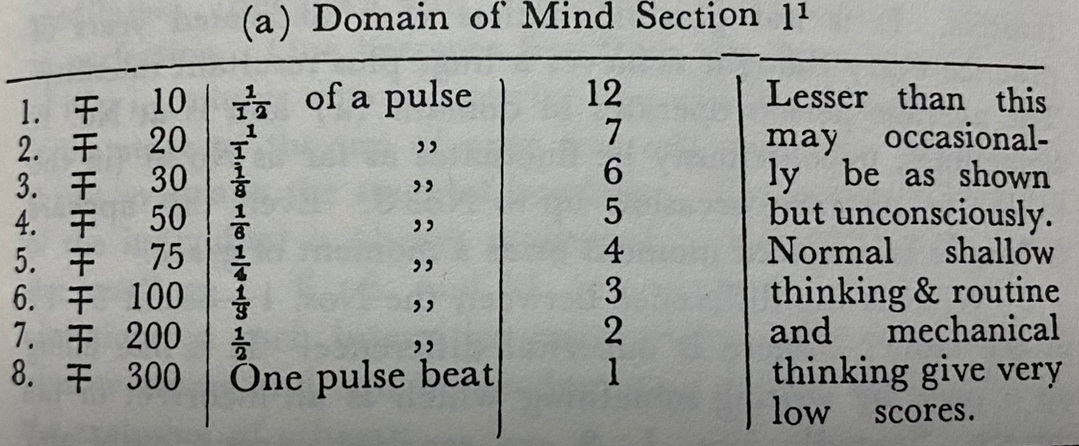
\includegraphics[width=0.9\linewidth,keepaspectratio]{images/zenyoga3}
	\end{center}
	
1st row, in 1 pulse, usually you get 12 thoughts, there you get 10 zenyoga points. If you get 1 thoughts per pulse (last row), then you get 300 points. 3SRB way is to reduce thoughts per pulse. Saving energy needed to decode those many thoughts.

\end{frame}

%%%%%%%%%%%%%%%%%%%%%%%%%%%%%%%%%%%%%%%%%%%%%%%%%%%%%%%%%%%%%%%%
\begin{frame}[fragile]\frametitle{Thoughts per Pulse}
	\begin{center}
	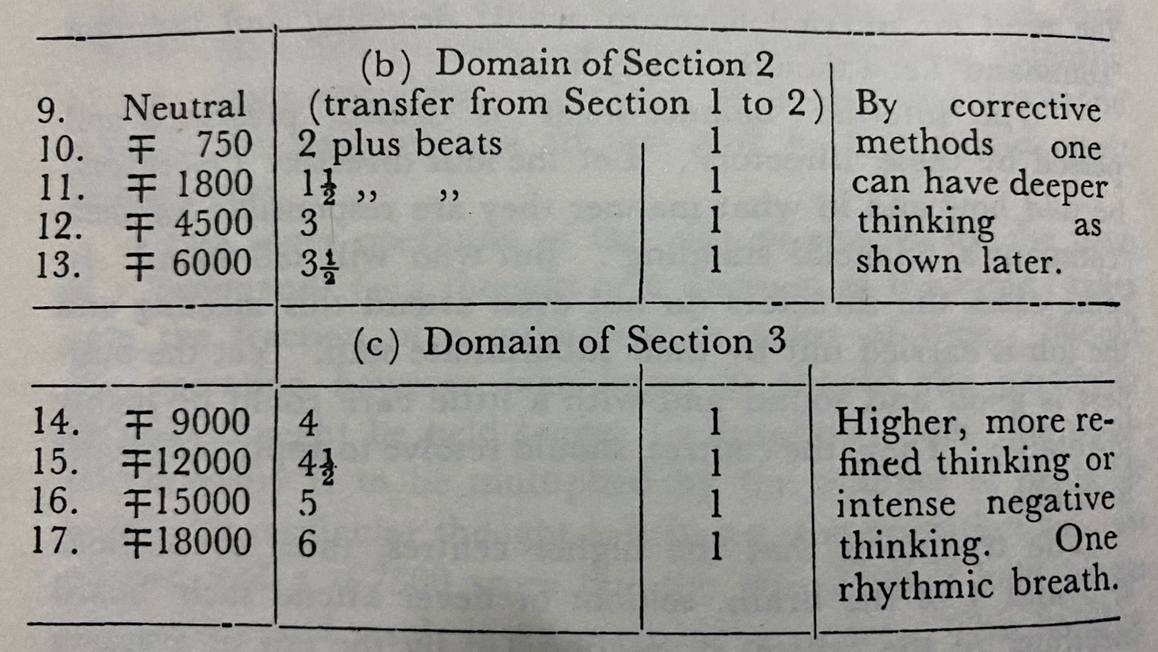
\includegraphics[width=0.9\linewidth,keepaspectratio]{images/zenyoga4}
	\end{center}
	
Reaching CSS you can hold 1 thought for 2-3-6 pulses.

\end{frame}

%%%%%%%%%%%%%%%%%%%%%%%%%%%%%%%%%%%%%%%%%%%%%%%%%%%%%%%%%%%%%%%%
\begin{frame}[fragile]\frametitle{Energy Drain and Thought Frequency}
    \begin{itemize}
        \item High thought-decoding rate exhausts mental and physical energy.
        \item An average person decodes approximately 51,000 thoughts per hour.
        \item Unconscious impulses from the five senses contribute to this high volume.
    \end{itemize}
\end{frame}

%%%%%%%%%%%%%%%%%%%%%%%%%%%%%%%%%%%%%%%%%%%%%%%%%%%%%%%%%%%%%%%%
\begin{frame}[fragile]\frametitle{Reducing Thought Frequency for Greater Intensity}
    \begin{itemize}
        \item Reducing thought frequency increases resultant intensity.
        \item Focus on breathing techniques, especially Three-Step Breathing, to slow down thought frequency.
        \item Slower frequency enhances mental clarity and reserves energy for higher purposes.
    \end{itemize}
\end{frame}

%%%%%%%%%%%%%%%%%%%%%%%%%%%%%%%%%%%%%%%%%%%%%%%%%%%%%%%%%%%%%%%%
\begin{frame}[fragile]\frametitle{Role of Heartbeat and Breathing in Thought Decoding}
    \begin{itemize}
        \item Thought decoding links to heartbeat and pulse frequency.
        \item Normal pulse rate allows decoding at a slower, more sustainable pace.
        \item Breathing practices help normalize pulse, stabilizing thought processes.
    \end{itemize}
\end{frame}

%%%%%%%%%%%%%%%%%%%%%%%%%%%%%%%%%%%%%%%%%%%%%%%%%%%%%%%%%%%%%%%%
\begin{frame}[fragile]\frametitle{Three-Step Breathing for Mental Calm}
    \begin{itemize}
        \item Three-Step Breathing helps in regulating the pulse to an ideal rate of 72 beats per minute.
        \item Reduces thought frequency, allowing energy conservation.
        \item Aids in gathering and storing Zen Yoga units effectively.
    \end{itemize}
\end{frame}

%%%%%%%%%%%%%%%%%%%%%%%%%%%%%%%%%%%%%%%%%%%%%%%%%%%%%%%%%%%%%%%%
\begin{frame}[fragile]\frametitle{Advanced Sections of the Mind}
    \begin{itemize}
        \item Sections 2, 3, and 4 of the mind require deeper thought regulation.
        \item Higher sections enable more intense thought folding per pulse.
        \item Advanced levels are only accessible with critical mastery of thought and pulse control.
    \end{itemize}
\end{frame}

%%%%%%%%%%%%%%%%%%%%%%%%%%%%%%%%%%%%%%%%%%%%%%%%%%%%%%%%%%%%%%%%
\begin{frame}[fragile]\frametitle{Section 2 Thought Decoding}
    \begin{itemize}
        \item As frequency reduces, thoughts fold into fewer pulses.
        \item Section 2 enables gathering up to 750 units of resultant intensity.
        \item Progressing beyond Section 1 requires substantial reduction in thought frequency.
    \end{itemize}
\end{frame}

%%%%%%%%%%%%%%%%%%%%%%%%%%%%%%%%%%%%%%%%%%%%%%%%%%%%%%%%%%%%%%%%
\begin{frame}[fragile]\frametitle{Zen Yoga Unit Collection in Higher Mind Sections}
    \begin{itemize}
        \item Mind sections gather specific intensities based on decoding frequency.
        \item Higher sections (3 and 4) allow folding of thoughts over multiple pulses, enhancing intensity.
        \item Advanced breathing and pulse control lead to refined positive or negative unit collection.
    \end{itemize}
\end{frame}

%%%%%%%%%%%%%%%%%%%%%%%%%%%%%%%%%%%%%%%%%%%%%%%%%%%%%%%%%%%%%%%%
\begin{frame}[fragile]\frametitle{Practical Application of Three-Step Breathing}
    \begin{itemize}
        \item Dedicate 10-15 minutes daily to Three-Step Breathing.
        \item Practice reduces unnecessary thoughts and energy drain.
        \item Regular practice aligns pulse and thought rates, conserving mental and physical energy.
    \end{itemize}
\end{frame}

%%%%%%%%%%%%%%%%%%%%%%%%%%%%%%%%%%%%%%%%%%%%%%%%%%%%%%%%%%%%%%%%
\begin{frame}[fragile]\frametitle{Conclusion: Evolving Through Zen Yoga}
    \begin{itemize}
        \item Zen Yoga emphasizes reducing thought frequency to achieve deeper mental states.
        \item Regulated pulse and breathing stabilize mental processes, making higher mind sections accessible.
        \item Mastery in thought control allows for Zen Yoga units to transform into positive, enduring energy.
    \end{itemize}
\end{frame}

%%%%%%%%%%%%%%%%%%%%%%%%%%%%%%%%%%%%%%%%%%%%%%%%%%%%%%%%%%%%%%%%
\begin{frame}[fragile]\frametitle{}
\begin{center}
{\Large Chapter 11: Use of Free Will in Trifles }
\end{center}
\end{frame}

%%%%%%%%%%%%%%%%%%%%%%%%%%%%%%%%%%%%%%%%%%%%%%%%%%%%%%%%%%%%%%%%
\begin{frame}[fragile]\frametitle{Use of Free Will and False Choices}
    \begin{itemize}
        \item Discussion on free will and how humans exercise it.
        \item Zenyoga emphasizes utilizing free will for spiritual growth.
        \item Importance of making conscious choices that align with life's purpose.
    \end{itemize}
\end{frame}

%%%%%%%%%%%%%%%%%%%%%%%%%%%%%%%%%%%%%%%%%%%%%%%%%%%%%%%%%%%%%%%%
\begin{frame}[fragile]\frametitle{Yoga's Eight Limbs}
    \begin{itemize}
        \item Zenyoga introduces the eight limbs of Yoga as steps toward enlightenment.
        \item Key stages: Yama, Niyama, Asana, Pranayama, Pratyahara, Dharana, Dhyana, Samadhi. यम नियम आसन प्राणायाम प्रत्याहार धारणा ध्यान समाधी 
        \item Final three stages focus on concentration, meditation, and transcendent union.
    \end{itemize}
\end{frame}

%%%%%%%%%%%%%%%%%%%%%%%%%%%%%%%%%%%%%%%%%%%%%%%%%%%%%%%%%%%%%%%%
\begin{frame}[fragile]\frametitle{Self-Discipline and Habit Formation}
    \begin{itemize}
        \item Yama, Niyama, Asana, and Pranayama यम नियम आसन प्राणायाम promote self-discipline in daily habits.
        \item Moderation in all activities, including eating and sleeping, is essential.
        \item Overindulgence affects physical and spiritual growth, slowing progress.
    \end{itemize}
\end{frame}

%%%%%%%%%%%%%%%%%%%%%%%%%%%%%%%%%%%%%%%%%%%%%%%%%%%%%%%%%%%%%%%%
\begin{frame}[fragile]\frametitle{Pratyahara – Withdrawal of Senses}
    \begin{itemize}
        \item Pratyahara प्रत्याहार is the stage of withdrawing from sensory distractions.
        \item Achieving this step fosters self-awareness beyond the physical body.
        \item It prepares the mind for deeper states of meditation.
    \end{itemize}
\end{frame}

%%%%%%%%%%%%%%%%%%%%%%%%%%%%%%%%%%%%%%%%%%%%%%%%%%%%%%%%%%%%%%%%
\begin{frame}[fragile]\frametitle{Role of Moderation in Daily Activities}
    \begin{itemize}
        \item Zenyoga emphasizes moderation in food, sleep, and all daily activities.
        \item Excess in any aspect leads to negative effects on body and mind.
        \item "Disinfection Chamber" approach: a disciplined boundary for actions.
    \end{itemize}
\end{frame}

%%%%%%%%%%%%%%%%%%%%%%%%%%%%%%%%%%%%%%%%%%%%%%%%%%%%%%%%%%%%%%%%
\begin{frame}[fragile]\frametitle{Understanding True Free Will}
    \begin{itemize}
        \item Misinterpretation of free will often leads to impulsive actions.
        \item Zenyoga teaches discerning right actions that contribute to spiritual growth.
        \item Avoid actions solely for temporary pleasures that detract from growth.
    \end{itemize}
\end{frame}

%%%%%%%%%%%%%%%%%%%%%%%%%%%%%%%%%%%%%%%%%%%%%%%%%%%%%%%%%%%%%%%%
\begin{frame}[fragile]\frametitle{Addictions and Misuse of Free Will}
    \begin{itemize}
        \item Addictions hinder spiritual and personal growth.
        \item Zenyoga addresses overcoming habits like overeating, substance use, and excessive sleep.
        \item Self-awareness and mindful action are essential to overcoming these patterns.
    \end{itemize}
\end{frame}

%%%%%%%%%%%%%%%%%%%%%%%%%%%%%%%%%%%%%%%%%%%%%%%%%%%%%%%%%%%%%%%%
\begin{frame}[fragile]\frametitle{Mind and Breath Control}
    \begin{itemize}
        \item Breath awareness is crucial for mental clarity and spiritual well-being.
        \item Optimal breathing frequency affects mental stability and thought quality.
        \item Nose breathing is recommended over mouth breathing for health and mental focus.
    \end{itemize}
\end{frame}

%%%%%%%%%%%%%%%%%%%%%%%%%%%%%%%%%%%%%%%%%%%%%%%%%%%%%%%%%%%%%%%%
\begin{frame}[fragile]\frametitle{Quality of Thoughts and Diet}
    \begin{itemize}
        \item Zenyoga highlights the connection between diet and quality of thoughts.
        \item Consumption of natural, balanced foods promotes positive, clear thoughts.
        \item Tamasik (heavy) foods tend to generate lethargic, negative thoughts.
    \end{itemize}
\end{frame}

%%%%%%%%%%%%%%%%%%%%%%%%%%%%%%%%%%%%%%%%%%%%%%%%%%%%%%%%%%%%%%%%
\begin{frame}[fragile]\frametitle{Life and Spiritual Journey Alignment}
    \begin{itemize}
        \item Zenyoga aims to harmonize physical habits with spiritual goals.
        \item Thoughtful habits and balanced choices lead to sustained growth.
        \item Recognizing the impact of actions today on future well-being.
    \end{itemize}
\end{frame}


%%%%%%%%%%%%%%%%%%%%%%%%%%%%%%%%%%%%%%%%%%%%%%%%%%%%%%%%%%%%%%%%
\begin{frame}[fragile]\frametitle{}
\begin{center}
{\Large Chapter 12: Corrective Methods In Daily Living }
\end{center}
\end{frame}

%%%%%%%%%%%%%%%%%%%%%%%%%%%%%%%%%%%%%%%%%%%%%%%%%%%%%%%%%%%%%%%%
\begin{frame}[fragile]\frametitle{Corrective Methods in Daily Living}
    \begin{itemize}
        \item The chapter discusses corrective methods in daily activities essential for survival.
        \item Focus on understanding common errors in daily actions and the correct approaches.
        \item Main topics include:
        \begin{itemize}
            \item Food and Drink
            \item Breath (Prana प्राण)
            \item Sensory Inputs and Thought Generation
        \end{itemize}
    \end{itemize}
\end{frame}

%%%%%%%%%%%%%%%%%%%%%%%%%%%%%%%%%%%%%%%%%%%%%%%%%%%%%%%%%%%%%%%%
\begin{frame}[fragile]\frametitle{Food and Drink: Mindful Consumption}
    \begin{itemize}
        \item Avoid preconceptions about vegetarian vs. non-vegetarian food.
        \item Choose foods that are easy for the body to digest.
        \item Maintain a calm mind while eating; express gratitude for the sustenance.
        \item Young individuals (below 21 years) may consume freely due to growth needs.
        \item For adults, focus on maintenance, replacing old cells, and restoring energy levels.
    \end{itemize}
\end{frame}

%%%%%%%%%%%%%%%%%%%%%%%%%%%%%%%%%%%%%%%%%%%%%%%%%%%%%%%%%%%%%%%%
\begin{frame}[fragile]\frametitle{Eating Habits for Health}
    \begin{itemize}
        \item Gradually reduce food quantity if eating multiple times a day.
        \item Avoid eating before 10:00 AM; limit eating times between 10:00 AM and 4:00 PM.
        \item Reducing food quantity can lead to increased energy and lighter body sensations.
        \item Reduce food intake mindfully over time for sustainable change.
    \end{itemize}
\end{frame}

%%%%%%%%%%%%%%%%%%%%%%%%%%%%%%%%%%%%%%%%%%%%%%%%%%%%%%%%%%%%%%%%
\begin{frame}[fragile]\frametitle{Managing Energy and Reducing Food Needs}
    \begin{itemize}
        \item Energy drains from mental, sensory, and physical activities increase food and sleep needs.
        \item Conserving energy can lead to reduced food and sleep requirements.
        \item With reduced energy drain, fewer meals and less sleep can still maintain high energy.
    \end{itemize}
\end{frame}

%%%%%%%%%%%%%%%%%%%%%%%%%%%%%%%%%%%%%%%%%%%%%%%%%%%%%%%%%%%%%%%%
\begin{frame}[fragile]\frametitle{Personal Experimentation with Food Quantity}
    \begin{itemize}
        \item Gradually reduced meal size from five rotis to two or three without health effects.
        \item Evening meals are taken early to reduce body load, improving energy levels and reducing sleep needs.
        \item Experimenting over several years has shown no decline in health with reduced quantity.
    \end{itemize}
\end{frame}

%%%%%%%%%%%%%%%%%%%%%%%%%%%%%%%%%%%%%%%%%%%%%%%%%%%%%%%%%%%%%%%%
\begin{frame}[fragile]\frametitle{Drinking: The Ideal Choice}
    \begin{itemize}
        \item Water is the best drink for hydration.
        \item Avoid alcohol due to its harmful effects on body cells and organs.
        \item Keep the body energized with simple, easily digestible food and clean water.
    \end{itemize}
\end{frame}

%%%%%%%%%%%%%%%%%%%%%%%%%%%%%%%%%%%%%%%%%%%%%%%%%%%%%%%%%%%%%%%%
\begin{frame}[fragile]\frametitle{Introduction to Rhythmic Breathing}
    \begin{itemize}
        \item Importance of breathing rhythm for overall well-being.
        \item Rhythmic breathing method introduced to correct disrupted breathing.
        \item Inspired by natural breathing patterns observed in infants.
    \end{itemize}
\end{frame}

%%%%%%%%%%%%%%%%%%%%%%%%%%%%%%%%%%%%%%%%%%%%%%%%%%%%%%%%%%%%%%%%
\begin{frame}[fragile]\frametitle{Step 1: Focus on Technique}
    \begin{itemize}
        \item Emphasize natural breathing rhythm.
        \item Use a heavy book on the abdomen to monitor abdominal movement.
        \item Breathe through the nose to direct air into the lungs.
        \item Minimize chest movement to encourage deep lung expansion.
    \end{itemize}
\end{frame}

%%%%%%%%%%%%%%%%%%%%%%%%%%%%%%%%%%%%%%%%%%%%%%%%%%%%%%%%%%%%%%%%
\begin{frame}[fragile]\frametitle{Step 2: Focus on Volume}
    \begin{itemize}
        \item Concentrate on filling the lungs completely.
        \item Practice against a wall with hands placed upwards to open the chest.
        \item Learn to increase air volume in each breath cycle.
        \item Maintain focus on proper lung expansion.
    \end{itemize}
\end{frame}

%%%%%%%%%%%%%%%%%%%%%%%%%%%%%%%%%%%%%%%%%%%%%%%%%%%%%%%%%%%%%%%%
\begin{frame}[fragile]\frametitle{Step 3: Natural Rhythm}
    \begin{itemize}
        \item Combine techniques from Steps 1 and 2.
        \item Breathing aligns with natural, relaxed rhythm.
        \item Practicing for 6+ months leads to unconscious mastery.
        \item Achieve lower heart and breath rates, indicating improved calmness.
    \end{itemize}
\end{frame}

%%%%%%%%%%%%%%%%%%%%%%%%%%%%%%%%%%%%%%%%%%%%%%%%%%%%%%%%%%%%%%%%
\begin{frame}[fragile]\frametitle{Benefits of Rhythmic Breathing Practice}
    \begin{itemize}
        \item Reduced irritability and stress response.
        \item Enhanced mental clarity and focus.
        \item Greater control over emotional responses.
        \item Improved physical and mental resilience in daily life.
    \end{itemize}
\end{frame}

%%%%%%%%%%%%%%%%%%%%%%%%%%%%%%%%%%%%%%%%%%%%%%%%%%%%%%%%%%%%%%%%
\begin{frame}[fragile]\frametitle{Not Pranayama, but a Pre-Practice}
    \begin{itemize}
        \item Rhythmic breathing is not Pranayama प्राणायाम.
        \item Suitable for those at preliminary stages of breathing practice.
        \item Focuses on rhythm and volume before advancing to Pranayama.
    \end{itemize}
\end{frame}

%%%%%%%%%%%%%%%%%%%%%%%%%%%%%%%%%%%%%%%%%%%%%%%%%%%%%%%%%%%%%%%%
\begin{frame}[fragile]\frametitle{}
\begin{center}
{\Large Chapter 13: Progress on The Path }
\end{center}
\end{frame}

%%%%%%%%%%%%%%%%%%%%%%%%%%%%%%%%%%%%%%%%%%%%%%%%%%%%%%%%%%%%%%%%
\begin{frame}[fragile]\frametitle{Progress on the Path}
    \begin{itemize}
        \item This chapter, titled "Progress on the Path," encourages mindful eating practices.
        \item Saher emphasizes sharing this knowledge with others for a collective improvement in life and mental well-being.
        \item Previous chapters discussed mindful eating and awareness of sensory inputs that impact our thoughts.
    \end{itemize}
\end{frame}

%%%%%%%%%%%%%%%%%%%%%%%%%%%%%%%%%%%%%%%%%%%%%%%%%%%%%%%%%%%%%%%%
\begin{frame}[fragile]\frametitle{Mindful Eating Practices}
    \begin{itemize}
        \item Focus on silence while eating, avoiding distractions like discussions, TV, or phones.
        \item Cultivate gratitude for the food by honoring it before eating.
        \item Mindfulness in eating affects both thought processes and internal mechanisms.
    \end{itemize}
\end{frame}

%%%%%%%%%%%%%%%%%%%%%%%%%%%%%%%%%%%%%%%%%%%%%%%%%%%%%%%%%%%%%%%%
\begin{frame}[fragile]\frametitle{Impact of Food on Thoughts and Body}
    \begin{itemize}
        \item Food quality influences thoughts and replaces old cells with new ones, aligned with mindful vibrations.
        \item Over time, mindful eating brings significant health and mental benefits, facilitating internal cleansing.
        \item Saher advises eating with "deliberate mindfulness" for a transformative effect on thoughts and body cells.
    \end{itemize}
\end{frame}

%%%%%%%%%%%%%%%%%%%%%%%%%%%%%%%%%%%%%%%%%%%%%%%%%%%%%%%%%%%%%%%%
\begin{frame}[fragile]\frametitle{Breaking the Cycle of Mindless Consumption}
    \begin{itemize}
        \item Avoid passive habits like watching TV or engaging in conversations while eating.
        \item Such distractions during meals influence thought quality and impact cellular regeneration.
        \item Focus on mindful eating to prevent unconscious absorption of negative traits from violent or aggressive media.
    \end{itemize}
\end{frame}

%%%%%%%%%%%%%%%%%%%%%%%%%%%%%%%%%%%%%%%%%%%%%%%%%%%%%%%%%%%%%%%%
\begin{frame}[fragile]\frametitle{Mindful Food Choices}
    \begin{itemize}
        \item Saher suggests observing how food affects the body and choosing meals accordingly.
        \item Eat simple, nutritious food that suits your body type, limiting tamasic (dullness-inducing) foods.
        \item Observe how different foods influence thoughts and energy levels over time.
    \end{itemize}
\end{frame}

%%%%%%%%%%%%%%%%%%%%%%%%%%%%%%%%%%%%%%%%%%%%%%%%%%%%%%%%%%%%%%%%
\begin{frame}[fragile]\frametitle{Portion Control and Gradual Adjustment}
    \begin{itemize}
        \item Saher advises eating only the required amount: one morsel per hour or a total of 24 morsels for a day.
        \item Gradually reduce food quantity if consuming multiple meals a day.
        \item Aim to practice mindful, focused eating over time for greater self-control and energy conservation.
    \end{itemize}
\end{frame}

%%%%%%%%%%%%%%%%%%%%%%%%%%%%%%%%%%%%%%%%%%%%%%%%%%%%%%%%%%%%%%%%
\begin{frame}[fragile]\frametitle{The Role of Self-Observation}
    \begin{itemize}
        \item Practice "depth-watching" to become aware of personal weaknesses and work on them over time.
        \item Focus on specific weaknesses for one month to gradually eliminate them.
        \item Dedication and awareness in eating help achieve long-term internal transformation.
    \end{itemize}
\end{frame}

%%%%%%%%%%%%%%%%%%%%%%%%%%%%%%%%%%%%%%%%%%%%%%%%%%%%%%%%%%%%%%%%
\begin{frame}[fragile]\frametitle{Internal Work as Social Contribution}
    \begin{itemize}
        \item The greatest social work is to transform oneself through mindful practices.
        \item Change in one's own thought process has a broader social impact.
        \item Self-transformation through conscious living is a valuable contribution to society.
    \end{itemize}
\end{frame}

%%%%%%%%%%%%%%%%%%%%%%%%%%%%%%%%%%%%%%%%%%%%%%%%%%%%%%%%%%%%%%%%
\begin{frame}[fragile]\frametitle{Preparation for Meditation}
    \begin{itemize}
        \item Meditation should not be approached superficially; it requires preparation.
        \item Start with refining food intake, self-observation, and rhythmic breathing.
        \item Attempting meditation without preparation will yield minimal benefits.
    \end{itemize}
\end{frame}

%%%%%%%%%%%%%%%%%%%%%%%%%%%%%%%%%%%%%%%%%%%%%%%%%%%%%%%%%%%%%%%%
\begin{frame}[fragile]\frametitle{Final Thoughts on the Path}
    \begin{itemize}
        \item Saher emphasizes the importance of gradual and committed practice on the path to transformation.
        \item Mindful eating, breathing exercises, and self-discipline form a foundational base for deeper practices.
        \item Focus on these preliminary steps to truly progress in meditation and self-awareness.
    \end{itemize}
\end{frame}


%%%%%%%%%%%%%%%%%%%%%%%%%%%%%%%%%%%%%%%%%%%%%%%%%%%%%%%%%%%%%%%%
\begin{frame}[fragile]\frametitle{}
\begin{center}
{\Large Chapter 14: Will-Force }
\end{center}
\end{frame}

%%%%%%%%%%%%%%%%%%%%%%%%%%%%%%%%%%%%%%%%%%%%%%%%%%%%%%%%%%%%%%%%
\begin{frame}[fragile]\frametitle{Introduction to Will Force}
    \begin{itemize}
        \item The concept of \textbf{will force} vs. \textbf{free will} is discussed.
        \item Unlike physical force, true will doesn't require forceful application.
        \item Will flows effortlessly when aligned with one's inner self.
    \end{itemize}
\end{frame}

%%%%%%%%%%%%%%%%%%%%%%%%%%%%%%%%%%%%%%%%%%%%%%%%%%%%%%%%%%%%%%%%
\begin{frame}[fragile]\frametitle{Understanding Sin and Negative Vibrations}
    \begin{itemize}
        \item Actions driven by \textbf{negative tendencies} are considered sins.
        \item Negative vibrations dominate one's centers, leading to negative actions.
        \item Sinful acts arise when these centers become imbalanced.
    \end{itemize}
\end{frame}

%%%%%%%%%%%%%%%%%%%%%%%%%%%%%%%%%%%%%%%%%%%%%%%%%%%%%%%%%%%%%%%%
\begin{frame}[fragile]\frametitle{Corrective Methods and Transformation}
    \begin{itemize}
        \item Transformation can occur through \textbf{three-step rhythmic breathing} and awareness.
        \item Awareness can cleanse one's negative actions, similar to Angulimala after meeting Buddha.
        \item Transformation of thought processes is key to cleansing life.
    \end{itemize}
\end{frame}

%%%%%%%%%%%%%%%%%%%%%%%%%%%%%%%%%%%%%%%%%%%%%%%%%%%%%%%%%%%%%%%%
\begin{frame}[fragile]\frametitle{Role of Free Will in Evolution}
    \begin{itemize}
        \item At critical stages, one learns to use free will wisely.
        \item Negative vibrations are controlled, enabling \textbf{right action and thought}.
        \item Free will guides one's life towards meaningful growth.
    \end{itemize}
\end{frame}

%%%%%%%%%%%%%%%%%%%%%%%%%%%%%%%%%%%%%%%%%%%%%%%%%%%%%%%%%%%%%%%%
\begin{frame}[fragile]\frametitle{Sustainability of Will Force}
    \begin{itemize}
        \item Will force alone cannot sustain life changes for long.
        \item Transformation through will requires \textbf{gradual, steady practice}.
        \item Difference between humans and animals lies in the ability to make conscious choices.
    \end{itemize}
\end{frame}

%%%%%%%%%%%%%%%%%%%%%%%%%%%%%%%%%%%%%%%%%%%%%%%%%%%%%%%%%%%%%%%%
\begin{frame}[fragile]\frametitle{Importance of the I-Center}
    \begin{itemize}
        \item The \textbf{I-center} has the highest intensity among centers.
        \item Its alignment with other centers enhances positive vibrations.
        \item With harmony across centers, transformation becomes effortless.
    \end{itemize}
\end{frame}

%%%%%%%%%%%%%%%%%%%%%%%%%%%%%%%%%%%%%%%%%%%%%%%%%%%%%%%%%%%%%%%%
\begin{frame}[fragile]\frametitle{Aligning Desires and Will}
    \begin{itemize}
        \item Will power is often confused with \textbf{desire control}.
        \item True will force requires alignment of one’s internal centers.
        \item Alignment is achieved through consistent \textbf{corrective practices}.
    \end{itemize}
\end{frame}

%%%%%%%%%%%%%%%%%%%%%%%%%%%%%%%%%%%%%%%%%%%%%%%%%%%%%%%%%%%%%%%%
\begin{frame}[fragile]\frametitle{Reflection and Inner Rhythm}
    \begin{itemize}
        \item Reflection on the \textbf{inner rhythm} helps align body, mind, and will.
        \item Questions to ponder: What is my inner rhythm? How do my will and cells act in harmony?
        \item This book aims to guide one towards discovering the right path.
    \end{itemize}
\end{frame}


%%%%%%%%%%%%%%%%%%%%%%%%%%%%%%%%%%%%%%%%%%%%%%%%%%%%%%%%%%%%%%%%
\begin{frame}[fragile]\frametitle{}
\begin{center}
{\Large Chapter 15: The Internal Non-equilibrium of the Centers  }
\end{center}
\end{frame}

%%%%%%%%%%%%%%%%%%%%%%%%%%%%%%%%%%%%%%%%%%%%%%%%%%%%%%%%%%%%%%%%
\begin{frame}[fragile]\frametitle{The Internal Non-Equilibrium of the Centers}
    \begin{itemize}
        \item The chapter discusses the non-equilibrium among our inner centers: \textbf{I-center}, \textbf{S-center}, \textbf{M-center}, and \textbf{E-center}.
        \item Each center has a specific intensity and relationship with the others.
        \item Equilibrium among these centers is essential for effective decision-making and action.
    \end{itemize}
\end{frame}

%%%%%%%%%%%%%%%%%%%%%%%%%%%%%%%%%%%%%%%%%%%%%%%%%%%%%%%%%%%%%%%%
\begin{frame}[fragile]\frametitle{Importance of Center Alignment}
    \begin{itemize}
        \item Decisions often fail when there is misalignment between the I-center and other centers.
        \item An unbalanced center configuration leads to indecisiveness and inconsistency in executing resolutions.
        \item Alignment ensures that body and mind work in harmony towards a set goal.
    \end{itemize}
\end{frame}

%%%%%%%%%%%%%%%%%%%%%%%%%%%%%%%%%%%%%%%%%%%%%%%%%%%%%%%%%%%%%%%%
\begin{frame}[fragile]\frametitle{Example of Misalignment}
    \begin{itemize}
        \item Example: Deciding to wake up at 4 AM but failing due to lack of alignment.
        \item The I-center initiates the decision, but other centers resist due to habitual preferences.
        \item This internal conflict often leads to snoozing the alarm, ultimately failing the initial goal.
    \end{itemize}
\end{frame}

%%%%%%%%%%%%%%%%%%%%%%%%%%%%%%%%%%%%%%%%%%%%%%%%%%%%%%%%%%%%%%%%
\begin{frame}[fragile]\frametitle{Example of Proper Alignment}
    \begin{itemize}
        \item When all centers are aligned, decisions are executed smoothly.
        \item Example: Excitement to go on a picnic or play sports causes the body to wake up early without resistance.
        \item Alignment creates a seamless execution of plans, as seen in joyful activities.
    \end{itemize}
\end{frame}

%%%%%%%%%%%%%%%%%%%%%%%%%%%%%%%%%%%%%%%%%%%%%%%%%%%%%%%%%%%%%%%%
\begin{frame}[fragile]\frametitle{Achieving Center Equilibrium}
    \begin{itemize}
        \item Aligning I, S, M, and E-centers for interest in challenging tasks, like studies, can improve performance.
        \item Associating less enjoyable tasks with something rewarding creates internal balance.
        \item Such alignment removes resistance and enhances the ability to execute decisions effectively.
    \end{itemize}
\end{frame}

%%%%%%%%%%%%%%%%%%%%%%%%%%%%%%%%%%%%%%%%%%%%%%%%%%%%%%%%%%%%%%%%
\begin{frame}[fragile]\frametitle{Understanding Yourself}
    \begin{itemize}
        \item Understanding oneself is more beneficial than trying to understand others.
        \item Proper tuning within ourselves enhances interpersonal relationships and self-growth.
        \item Aligning our centers allows us to communicate and relate better with others.
    \end{itemize}
\end{frame}



%%%%%%%%%%%%%%%%%%%%%%%%%%%%%%%%%%%%%%%%%%%%%%%%%%%%%%%%%%%%%%%%
\begin{frame}[fragile]\frametitle{}
\begin{center}
{\Large Chapter 16: How Can We Restore The Internal Equilibrium of the Centers  }
\end{center}
\end{frame}

%%%%%%%%%%%%%%%%%%%%%%%%%%%%%%%%%%%%%%%%%%%%%%%%%%%%%%%%%%%%%%%%
\begin{frame}[fragile]\frametitle{Restoring Internal Equilibrium of Mind Centers}
    \begin{itemize}
        \item This chapter explores methods to restore the equilibrium of the mind’s centers.
        \item The harmony among these centers is essential for successful decision-making and habit formation.
    \end{itemize}
\end{frame}

%%%%%%%%%%%%%%%%%%%%%%%%%%%%%%%%%%%%%%%%%%%%%%%%%%%%%%%%%%%%%%%%
\begin{frame}[fragile]\frametitle{Overview of Mind Centers}
    \begin{itemize}
        \item There are seven main centers in the mind.
        \item The first center is divided into four parts: \textbf{I} (Intelligence), \textbf{S} (Sensibility), \textbf{I} (Impulse), and \textbf{M} (Mobility).
        \item These four components work together to produce actions and thoughts.
    \end{itemize}
\end{frame}

%%%%%%%%%%%%%%%%%%%%%%%%%%%%%%%%%%%%%%%%%%%%%%%%%%%%%%%%%%%%%%%%
\begin{frame}[fragile]\frametitle{Intuition Center}
    \begin{itemize}
        \item The second center is the Intuition Center, split into two parts: Section 2A and Section 2B.
        \item Section 2A governs autonomous bodily functions, including chemical reactions and neural activities.
        \item Section 2B, accessed through advanced mental training, is associated with critical thinking and deep insight.
    \end{itemize}
\end{frame}

%%%%%%%%%%%%%%%%%%%%%%%%%%%%%%%%%%%%%%%%%%%%%%%%%%%%%%%%%%%%%%%%
\begin{frame}[fragile]\frametitle{Higher Centers of the Mind}
    \begin{itemize}
        \item The third center operates at a molecular level, responsible for subtle perception and advanced mental capabilities.
        \item The fourth and final center, functioning on an electronic level, provides a deeper level of perception.
    \end{itemize}
\end{frame}

%%%%%%%%%%%%%%%%%%%%%%%%%%%%%%%%%%%%%%%%%%%%%%%%%%%%%%%%%%%%%%%%
\begin{frame}[fragile]\frametitle{Levels of Mind Perception}
    \begin{itemize}
        \item \textbf{Cellular Level}: Processes sensory information and produces thoughts based on basic perception.
        \item \textbf{Molecular Level}: Enables enhanced understanding and multi-dimensional perception of objects.
        \item \textbf{Electronic Level}: Allows insight into the core components of objects beyond surface perception.
    \end{itemize}
\end{frame}

%%%%%%%%%%%%%%%%%%%%%%%%%%%%%%%%%%%%%%%%%%%%%%%%%%%%%%%%%%%%%%%%
\begin{frame}[fragile]\frametitle{Maintaining Equilibrium}
    \begin{itemize}
        \item To maintain equilibrium, the \textbf{I Center} (Intelligence) must align with other centers before issuing commands.
        \item Misalignment among centers leads to conflicts, blocking effective action.
    \end{itemize}
\end{frame}

%%%%%%%%%%%%%%%%%%%%%%%%%%%%%%%%%%%%%%%%%%%%%%%%%%%%%%%%%%%%%%%%
\begin{frame}[fragile]\frametitle{Practical Approach to Center Alignment}
    \begin{itemize}
        \item Visualize tasks in advance to check for alignment with all centers.
        \item If a task conflicts with the preferences of any center, adjust the plan accordingly.
        \item For example, if morning study isn’t aligned, opt for an activity all centers agree upon, like physical exercise.
    \end{itemize}
\end{frame}

%%%%%%%%%%%%%%%%%%%%%%%%%%%%%%%%%%%%%%%%%%%%%%%%%%%%%%%%%%%%%%%%
\begin{frame}[fragile]\frametitle{Summary: Restoring Equilibrium}
    \begin{itemize}
        \item Restoring equilibrium requires understanding the functions and interrelations of the mind’s centers.
        \item Aligning tasks with the centers’ strengths supports consistent, harmonious actions and goals.
    \end{itemize}
\end{frame}


%%%%%%%%%%%%%%%%%%%%%%%%%%%%%%%%%%%%%%%%%%%%%%%%%%%%%%%%%%%%%%%%
\begin{frame}[fragile]\frametitle{Restoring Equilibrium of Centers}
    \begin{itemize}
        \item Discussion on restoring equilibrium of centers
        \item Importance of food practices and rhythmic breathing
        \item Aligning body and mind through three-step rhythmic breathing
    \end{itemize}
\end{frame}

%%%%%%%%%%%%%%%%%%%%%%%%%%%%%%%%%%%%%%%%%%%%%%%%%%%%%%%%%%%%%%%%
\begin{frame}[fragile]\frametitle{Challenges in Meditation}
    \begin{itemize}
        \item Common challenge: trying to stop thoughts during meditation
        \item Nature of the mind is to form pictures and process impulses
        \item Forcing the mind to stop this process is almost impossible
    \end{itemize}
\end{frame}

%%%%%%%%%%%%%%%%%%%%%%%%%%%%%%%%%%%%%%%%%%%%%%%%%%%%%%%%%%%%%%%%
\begin{frame}[fragile]\frametitle{Role of Mind Sections in Meditation}
    \begin{itemize}
        \item Section-1: Continuously forms pictures, difficult to stop
        \item Meditation requires activation of Section-2 for concentration
        \item Opening Section-2 enables deep concentration and meditation
    \end{itemize}
\end{frame}

%%%%%%%%%%%%%%%%%%%%%%%%%%%%%%%%%%%%%%%%%%%%%%%%%%%%%%%%%%%%%%%%
\begin{frame}[fragile]\frametitle{Observing Thoughts}
    \begin{itemize}
        \item Practice of observing thoughts rather than stopping them
        \item “Drip watching” technique to align thoughts and breathing
        \item Enables critical awareness and control over mental processes
    \end{itemize}
\end{frame}

%%%%%%%%%%%%%%%%%%%%%%%%%%%%%%%%%%%%%%%%%%%%%%%%%%%%%%%%%%%%%%%%
\begin{frame}[fragile]\frametitle{Interplay of Centers}
    \begin{itemize}
        \item Centers interact through positive, negative, and neutral phases
        \item Vertical and horizontal transfer of intensity between centers
        \item Visualization of center interactions as merging colors
    \end{itemize}
\end{frame}

%%%%%%%%%%%%%%%%%%%%%%%%%%%%%%%%%%%%%%%%%%%%%%%%%%%%%%%%%%%%%%%%
\begin{frame}[fragile]\frametitle{Impact of Mental Patterns on Health}
    \begin{itemize}
        \item Repeated mental patterns affect physical health
        \item Accumulation of negative intensities can deform cells
        \item Corrective measures through food practices and mindfulness
    \end{itemize}
\end{frame}

%%%%%%%%%%%%%%%%%%%%%%%%%%%%%%%%%%%%%%%%%%%%%%%%%%%%%%%%%%%%%%%%
\begin{frame}[fragile]\frametitle{Purpose of Corrective Practices}
    \begin{itemize}
        \item Benefits everyone, not just spiritually inclined individuals
        \item Helps in reducing suffering by aligning mind and body
        \item Improves relationships, work, and personal well-being
    \end{itemize}
\end{frame}

%%%%%%%%%%%%%%%%%%%%%%%%%%%%%%%%%%%%%%%%%%%%%%%%%%%%%%%%%%%%%%%%
\begin{frame}[fragile]\frametitle{Role of Section-1 and Section-2}
    \begin{itemize}
        \item Development of Section-2 enables deeper concentration
        \item Spiritual progress becomes automatic as Section-2 activates
        \item Insights from Section-2 are shared with Section-1
    \end{itemize}
\end{frame}

%%%%%%%%%%%%%%%%%%%%%%%%%%%%%%%%%%%%%%%%%%%%%%%%%%%%%%%%%%%%%%%%
\begin{frame}[fragile]\frametitle{Dreams and Insights}
    \begin{itemize}
        \item Section-1 reduces activity by 95\% during sleep
        \item Some dreams provide valuable insights when remembered
        \item Maintaining awareness in sleep can allow transfer of insights
    \end{itemize}
\end{frame}

%%%%%%%%%%%%%%%%%%%%%%%%%%%%%%%%%%%%%%%%%%%%%%%%%%%%%%%%%%%%%%%%
\begin{frame}[fragile]\frametitle{Yoga as the Process of Awakening}
    \begin{itemize}
        \item Meditation in awake state mirrors deep sleep awareness
        \item Yoga enables conscious practice of awareness and insight
        \item The beauty of yoga lies in merging deep rest with conscious focus
    \end{itemize}
\end{frame}


%%%%%%%%%%%%%%%%%%%%%%%%%%%%%%%%%%%%%%%%%%%%%%%%%%%%%%%%%%%%%%%%
\begin{frame}[fragile]\frametitle{}
\begin{center}
{\Large Chapter 17: What is the Purpose of Life and Birth?}
\end{center}
\end{frame}

%%%%%%%%%%%%%%%%%%%%%%%%%%%%%%%%%%%%%%%%%%%%%%%%%%%%%%%%%%%%%%%%
\begin{frame}[fragile]\frametitle{Purpose of Life and Birth}
    \begin{itemize}
        \item The essence of life and birth's purpose is central not only to this chapter but also to the entire first part of the book.
        \item Saher shares practical insights about life based on personal experience, emphasizing practices that bring real results when applied.
    \end{itemize}
\end{frame}

%%%%%%%%%%%%%%%%%%%%%%%%%%%%%%%%%%%%%%%%%%%%%%%%%%%%%%%%%%%%%%%%
\begin{frame}[fragile]\frametitle{Magic Formula for Life}
    \begin{itemize}
        \item Saher introduces a "magic formula": constantly ask yourself, \textit{"What is the purpose of life and birth?"}
        \item This question guides actions and decisions towards meaningful living, aligning activities with life's purpose.
    \end{itemize}
\end{frame}

%%%%%%%%%%%%%%%%%%%%%%%%%%%%%%%%%%%%%%%%%%%%%%%%%%%%%%%%%%%%%%%%
\begin{frame}[fragile]\frametitle{Human Existence and Purpose}
    \begin{itemize}
        \item Human life offers a unique opportunity to understand oneself deeply.
        \item Self-inquiry leads to answers about life, the universe, and our role within it.
        \item The human form allows for exploration beyond mere survival, towards inner knowledge.
    \end{itemize}
\end{frame}

%%%%%%%%%%%%%%%%%%%%%%%%%%%%%%%%%%%%%%%%%%%%%%%%%%%%%%%%%%%%%%%%
\begin{frame}[fragile]\frametitle{Balancing Material and Spiritual Life}
    \begin{itemize}
        \item Saher advises maintaining a balance between material and spiritual pursuits.
        \item Material well-being is necessary to support spiritual growth; neglecting it may hinder inner exploration.
    \end{itemize}
\end{frame}

%%%%%%%%%%%%%%%%%%%%%%%%%%%%%%%%%%%%%%%%%%%%%%%%%%%%%%%%%%%%%%%%
\begin{frame}[fragile]\frametitle{Practical Practices}
    \begin{itemize}
        \item Breathing exercises, disciplined eating, and regulated sleep help maintain a stable inner environment.
        \item These practices prevent crossing the "safety point," where emotions and thoughts lose control, similar to how a thermometer exceeds its limit.
    \end{itemize}
\end{frame}

%%%%%%%%%%%%%%%%%%%%%%%%%%%%%%%%%%%%%%%%%%%%%%%%%%%%%%%%%%%%%%%%
\begin{frame}[fragile]\frametitle{Avoiding Over-Indulgence}
    \begin{itemize}
        \item Excessive actions (over-eating, over-sleeping) disturb mental balance and lead to undesirable behaviors.
        \item Awareness in daily habits fosters control and supports spiritual and mental alignment.
    \end{itemize}
\end{frame}

%%%%%%%%%%%%%%%%%%%%%%%%%%%%%%%%%%%%%%%%%%%%%%%%%%%%%%%%%%%%%%%%
\begin{frame}[fragile]\frametitle{Impact of Consistent Practice}
    \begin{itemize}
        \item Consistent practice results in positive life changes that are noticeable in relationships, work, and overall outlook.
        \item Discipline across various aspects of life enhances self-improvement and stability.
    \end{itemize}
\end{frame}

%%%%%%%%%%%%%%%%%%%%%%%%%%%%%%%%%%%%%%%%%%%%%%%%%%%%%%%%%%%%%%%%
\begin{frame}[fragile]\frametitle{Self-Improvement and Spiritual Journey}
    \begin{itemize}
        \item Self-improvement is essential; spiritual practices, like immersion in "spiritual waters," purify the mind and thoughts.
        \item Each individual follows a unique path; Saher encourages reading and re-reading his teachings for deeper understanding.
    \end{itemize}
\end{frame}



%%%%%%%%%%%%%%%%%%%%%%%%%%%%%%%%%%%%%%%%%%%%%%%%%%%%%%%%%%%%%%%%
\begin{frame}[fragile]\frametitle{}
\begin{center}
{\Large Part II}
\end{center}
\end{frame}

%%%%%%%%%%%%%%%%%%%%%%%%%%%%%%%%%%%%%%%%%%%%%%%%%%%%%%%%%%%%%%%%
\begin{frame}[fragile]\frametitle{}
\begin{center}
{\Large Chapter 1: Pratyahara }
\end{center}
\end{frame}


%%%%%%%%%%%%%%%%%%%%%%%%%%%%%%%%%%%%%%%%%%%%%%%%%%%%%%%%%%%%%%%%
\begin{frame}[fragile]\frametitle{Introduction to Part Two}
    \begin{itemize}
        \item Part One covered foundational practices to control impulses, food habits, and sleep for reaching critical stages in self-discipline.
        \item Part Two begins with \textbf{Pratyahara}, the fifth step in Yoga.
        \item Preceded by Yama, Niyama, Asana, and Pranayama, these practices help one advance toward Pratyahara.
    \end{itemize}
\end{frame}

%%%%%%%%%%%%%%%%%%%%%%%%%%%%%%%%%%%%%%%%%%%%%%%%%%%%%%%%%%%%%%%%
\begin{frame}[fragile]\frametitle{The Concept of Pratyahara}
    \begin{itemize}
        \item Pratyahara is the withdrawal of the senses from external objects, enabling focus within.
        \item It is compared to crossing a river, moving from external practices (Yama, Niyama, etc.) toward deeper inner practices.
        \item Saher calls this state a 'no man's land' in the journey to higher stages of Yoga.
    \end{itemize}
\end{frame}

%%%%%%%%%%%%%%%%%%%%%%%%%%%%%%%%%%%%%%%%%%%%%%%%%%%%%%%%%%%%%%%%
\begin{frame}[fragile]\frametitle{Process and Significance of Pratyahara}
    \begin{itemize}
        \item Achieved by mastering Asana and Pranayama, Pratyahara regulates impulses in the body and brings control over vital energies.
        \item Helps to withdraw from sensory perceptions, leading to a balanced and energy-conserving mental state.
        \item Marks readiness for advanced concentration practices like Dharana, Dhyana, and Samadhi.
    \end{itemize}
\end{frame}

%%%%%%%%%%%%%%%%%%%%%%%%%%%%%%%%%%%%%%%%%%%%%%%%%%%%%%%%%%%%%%%%
\begin{frame}[fragile]\frametitle{Transition to Higher States}
    \begin{itemize}
        \item Pratyahara aligns mental faculties to achieve equilibrium, necessary for deeper stages of Yoga.
        \item Achieving a critical balance enables focus on minimal thoughts, conserving mental energy.
        \item Described as the mind's preparation to reach "escape velocity," similar to a rocket leaving Earth's gravitational pull.
    \end{itemize}
\end{frame}

%%%%%%%%%%%%%%%%%%%%%%%%%%%%%%%%%%%%%%%%%%%%%%%%%%%%%%%%%%%%%%%%
\begin{frame}[fragile]\frametitle{Reflection and Contemplation}
    \begin{itemize}
        \item At the end of each chapter, Saher prompts reflective questions to deepen understanding.
        \item Example: "What is the Supreme Truth, and how does it manifest on Earth?"
        \item These reflections aid in realizing inner truths and understanding the essence of mind and self.
    \end{itemize}
\end{frame}



%%%%%%%%%%%%%%%%%%%%%%%%%%%%%%%%%%%%%%%%%%%%%%%%%%%%%%%%%%%%%%%%
\begin{frame}[fragile]\frametitle{}
\begin{center}
{\Large Chapter 2: Self-Conquest }
\end{center}
\end{frame}

%%%%%%%%%%%%%%%%%%%%%%%%%%%%%%%%%%%%%%%%%%%%%%%%%%%%%%%%%%%%%%%%
\begin{frame}[fragile]\frametitle{Victory Over Self}
    \begin{itemize}
        \item In the previous chapter, we discussed *Pratyahara* - the stage of withdrawing the senses.
        \item This stage helps us transcend the physical body and realize that our mind is not limited to it.
        \item We learn to detach from our mind, understanding its capability to connect beyond the physical self.
    \end{itemize}
\end{frame}

%%%%%%%%%%%%%%%%%%%%%%%%%%%%%%%%%%%%%%%%%%%%%%%%%%%%%%%%%%%%%%%%
\begin{frame}[fragile]\frametitle{Control Over Mind and Practices}
    \begin{itemize}
        \item *Victory over self* implies complete control over the mind.
        \item Practicing *Yama*, *Niyama*, *Asana*, and *Pranayama* becomes crucial for regulating thoughts.
        \item These practices integrate into life, refining understanding of the mind's latent powers.
    \end{itemize}
\end{frame}

%%%%%%%%%%%%%%%%%%%%%%%%%%%%%%%%%%%%%%%%%%%%%%%%%%%%%%%%%%%%%%%%
\begin{frame}[fragile]\frametitle{Accessing Life-Giving Energy (Prana)}
    \begin{itemize}
        \item Prana, the energy permeating the universe, sustains life.
        \item By aligning with the universe's frequency, we tap into this life-giving energy.
        \item This alignment fills our cells with vitality, allowing us to feel the prana throughout the body.
    \end{itemize}
\end{frame}

%%%%%%%%%%%%%%%%%%%%%%%%%%%%%%%%%%%%%%%%%%%%%%%%%%%%%%%%%%%%%%%%
\begin{frame}[fragile]\frametitle{Thought Regulation and Energy Conservation}
    \begin{itemize}
        \item Reducing thought frequency through regulated breathing conserves mental energy.
        \item Lower thought frequency during practices enhances positive mental intensity.
        \item Stored energy facilitates faster progress in meditation and inner practices.
    \end{itemize}
\end{frame}

%%%%%%%%%%%%%%%%%%%%%%%%%%%%%%%%%%%%%%%%%%%%%%%%%%%%%%%%%%%%%%%%
\begin{frame}[fragile]\frametitle{Higher Consciousness and Detachment}
    \begin{itemize}
        \item With controlled senses, awareness of deeper aspects of life emerges.
        \item Detachment from one's shadow (ego) brings realization that the self-image is transient.
        \item The essence of this journey is separating oneself from the shadow of ego.
    \end{itemize}
\end{frame}

%%%%%%%%%%%%%%%%%%%%%%%%%%%%%%%%%%%%%%%%%%%%%%%%%%%%%%%%%%%%%%%%
\begin{frame}[fragile]\frametitle{Reflective Thought}
    \begin{itemize}
        \item *Thought for Reflection:* "How can I free myself from my own shadow?"
        \item This question urges detachment from the self-image and ego as part of spiritual growth.
    \end{itemize}
\end{frame}



%%%%%%%%%%%%%%%%%%%%%%%%%%%%%%%%%%%%%%%%%%%%%%%%%%%%%%%%%%%%%%%%
\begin{frame}[fragile]\frametitle{}
\begin{center}
{\Large Chapter 3: Understanding the laws of Spiritual Success }
\end{center}
\end{frame}


%%%%%%%%%%%%%%%%%%%%%%%%%%%%%%%%%%%%%%%%%%%%%%%%%%%%%%%%%%%%%%%%
\begin{frame}[fragile]\frametitle{Understanding with Spiritual Success}
    \begin{itemize}
        \item Spirituality involves opening all sections of the mind.
        \item Reaching the transcendental state (Samadhi) requires following certain laws.
        \item Merely achieving a critical stage doesn't guarantee opening of all mind sections.
        \item Consistent intensity in concentration and meditation is necessary.
    \end{itemize}
\end{frame}

%%%%%%%%%%%%%%%%%%%%%%%%%%%%%%%%%%%%%%%%%%%%%%%%%%%%%%%%%%%%%%%%
\begin{frame}[fragile]\frametitle{Analogy of a Rocket}
    \begin{itemize}
        \item Just as a rocket escapes Earth’s gravitational pull by reaching 25,000 mph, the mind must reach a critical stage.
        \item Achieving this critical stage requires collecting 201 Zenyoga units, a form of positive intensity energy.
        \item These units are accumulated through regular practice of Asanas and Pranayama.
    \end{itemize}
\end{frame}

%%%%%%%%%%%%%%%%%%%%%%%%%%%%%%%%%%%%%%%%%%%%%%%%%%%%%%%%%%%%%%%%
\begin{frame}[fragile]\frametitle{Aligning Mind Centers}
    \begin{itemize}
        \item Positive intensity aligns the centers of the mind, creating the 5:2:1 balance.
        \item Initially, humans experience a 2:4:8 ratio.
        \item Collecting 201 units enables the mind to reach a "critical setting stage."
        \item This stage allows the mind to transcend life’s gravitational pull.
    \end{itemize}
\end{frame}

%%%%%%%%%%%%%%%%%%%%%%%%%%%%%%%%%%%%%%%%%%%%%%%%%%%%%%%%%%%%%%%%
\begin{frame}[fragile]\frametitle{Attaining Pratyahara}
    \begin{itemize}
        \item Reaching the critical stage allows detachment from senses, achieving Pratyahara.
        \item Senses are the main ties binding life; withdrawing from them gives freedom.
        \item After Pratyahara, progress requires deepened concentration and meditation.
    \end{itemize}
\end{frame}

%%%%%%%%%%%%%%%%%%%%%%%%%%%%%%%%%%%%%%%%%%%%%%%%%%%%%%%%%%%%%%%%
\begin{frame}[fragile]\frametitle{Beyond Pratyahara: Avoiding Bondage}
    \begin{itemize}
        \item Even after Pratyahara, concentration and meditation are essential to avoid stagnation.
        \item New experiences may create attachments; progress demands transcending them.
        \item Awareness must be maintained to avoid getting stuck in the “gravitational pull” of experience.
    \end{itemize}
\end{frame}

%%%%%%%%%%%%%%%%%%%%%%%%%%%%%%%%%%%%%%%%%%%%%%%%%%%%%%%%%%%%%%%%
\begin{frame}[fragile]\frametitle{Supreme Creator Meditation}
    \begin{itemize}
        \item Focus on the thought of the Supreme Creator as the goal of the universe.
        \item Close your eyes, concentrate between the eyebrows, and enter a deep meditative state.
        \item This meditative focus allows merging with the Divine Power, the source of all creation.
    \end{itemize}
\end{frame}


%%%%%%%%%%%%%%%%%%%%%%%%%%%%%%%%%%%%%%%%%%%%%%%%%%%%%%%%%%%%%%%%
\begin{frame}[fragile]\frametitle{}
\begin{center}
{\Large Chapter 4: Glamour of Liberation from Bondage to the Ego }
\end{center}
\end{frame}

%%%%%%%%%%%%%%%%%%%%%%%%%%%%%%%%%%%%%%%%%%%%%%%%%%%%%%%%%%%%%%%%
\begin{frame}[fragile]\frametitle{Introduction}
    \begin{itemize}
        \item This chapter, titled "The Grammar of Liberation," discusses freeing oneself from the life force and advancing on the spiritual journey.
        \item It explores the stages of mind progression, specifically Section Three and Four of the mind.
    \end{itemize}
\end{frame}

%%%%%%%%%%%%%%%%%%%%%%%%%%%%%%%%%%%%%%%%%%%%%%%%%%%%%%%%%%%%%%%%
\begin{frame}[fragile]\frametitle{Stages of Liberation}
    \begin{itemize}
        \item Initially, liberation from life’s gravitational pull allows spiritual progression.
        \item As one progresses, certain psychic powers manifest, creating a sense of reaching cosmic consciousness.
        \item However, this stage is only an intermediate milestone, not the ultimate spiritual destination.
    \end{itemize}
\end{frame}

%%%%%%%%%%%%%%%%%%%%%%%%%%%%%%%%%%%%%%%%%%%%%%%%%%%%%%%%%%%%%%%%
\begin{frame}[fragile]\frametitle{The Glamor of Psychic Powers}
    \begin{itemize}
        \item Upon reaching Section Three, individuals may mistakenly believe they have achieved cosmic consciousness.
        \item P.J. Saher warns that these psychic abilities are temporary states, and one must continue the journey.
        \item The lure of powers can trap individuals in a “glamorous” orbit, creating a false sense of completion.
    \end{itemize}
\end{frame}

%%%%%%%%%%%%%%%%%%%%%%%%%%%%%%%%%%%%%%%%%%%%%%%%%%%%%%%%%%%%%%%%
\begin{frame}[fragile]\frametitle{Mind Centers: Junior and Senior Directors}
    \begin{itemize}
        \item Section Three is referred to as the Junior Managing Director of the mind.
        \item Section Four, known as the Senior Managing Director, offers higher wisdom and control.
        \item Achieving harmony between these sections is essential for true progress.
    \end{itemize}
\end{frame}

%%%%%%%%%%%%%%%%%%%%%%%%%%%%%%%%%%%%%%%%%%%%%%%%%%%%%%%%%%%%%%%%
\begin{frame}[fragile]\frametitle{Illusion of Spiritual Arrival}
    \begin{itemize}
        \item The glamour of psychic powers can cause individuals to believe they have reached their ultimate goal.
        \item Saher emphasizes the need for simplicity and humility, warning against the allure of temporary accomplishments.
        \item Many people start ashrams or spiritual practices at this stage, mistaking it for the end goal.
    \end{itemize}
\end{frame}

%%%%%%%%%%%%%%%%%%%%%%%%%%%%%%%%%%%%%%%%%%%%%%%%%%%%%%%%%%%%%%%%
\begin{frame}[fragile]\frametitle{The Purpose of Life and Work}
    \begin{itemize}
        \item True liberation lies in realizing the purpose of life, beyond temporary gains.
        \item One must consistently remind oneself of life’s purpose to avoid getting lost in superficial milestones.
        \item Continuous self-reflection strengthens resolve on the spiritual journey.
    \end{itemize}
\end{frame}

%%%%%%%%%%%%%%%%%%%%%%%%%%%%%%%%%%%%%%%%%%%%%%%%%%%%%%%%%%%%%%%%
\begin{frame}[fragile]\frametitle{Value of Prayer and Devotion}
    \begin{itemize}
        \item Devotion to the Divine reinforces resilience on the path to liberation.
        \item Saher suggests that genuine prayer and commitment to the divine purpose can summon universal support.
        \item Regular prayer deepens focus and aids in overcoming distractions along the journey.
    \end{itemize}
\end{frame}

%%%%%%%%%%%%%%%%%%%%%%%%%%%%%%%%%%%%%%%%%%%%%%%%%%%%%%%%%%%%%%%%
\begin{frame}[fragile]\frametitle{Conclusion: Beyond Glamour to True Liberation}
    \begin{itemize}
        \item Spiritual progress requires determination and awareness of life’s ultimate purpose.
        \item Temporary psychic experiences should not be mistaken for the final stage of liberation.
        \item Prayer, humility, and devotion guide one beyond illusions toward genuine spiritual attainment.
    \end{itemize}
\end{frame}




%%%%%%%%%%%%%%%%%%%%%%%%%%%%%%%%%%%%%%%%%%%%%%%%%%%%%%%%%%%%%%%%
\begin{frame}[fragile]\frametitle{}
\begin{center}
{\Large Chapter 5: Yoga Sutra in the Light of Our Understanding }
\end{center}
\end{frame}

%%%%%%%%%%%%%%%%%%%%%%%%%%%%%%%%%%%%%%%%%%%%%%%%%%%%%%%%%%%%%%%%
\begin{frame}[fragile]\frametitle{Yoga Sutras in the Light of Understanding}
    \begin{itemize}
        \item The previous chapter discussed the journey beyond section-free consciousness, entering a glamorous world of siddhis (spiritual powers).
        \item In this state, we can become attached to these powers, which can divert us from our true path.
        \item The key is to meditate in a way that guides us to section-4, helping us avoid getting trapped in this illusionary world.
    \end{itemize}
\end{frame}

%%%%%%%%%%%%%%%%%%%%%%%%%%%%%%%%%%%%%%%%%%%%%%%%%%%%%%%%%%%%%%%%
\begin{frame}[fragile]\frametitle{Avoiding Attachment to Siddhis}
    \begin{itemize}
        \item The goal is to free ourselves from attachment to the material world and life force, not to get stuck in the seductive orbit of siddhis.
        \item We must understand that true liberation requires us to transcend these distractions and focus on our true purpose.
        \item Only then can we be free from the cycle of birth and rebirth.
    \end{itemize}
\end{frame}

%%%%%%%%%%%%%%%%%%%%%%%%%%%%%%%%%%%%%%%%%%%%%%%%%%%%%%%%%%%%%%%%
\begin{frame}[fragile]\frametitle{Aligning Mind and Body with the Universe}
    \begin{itemize}
        \item When we practice regularly, our mind and body frequency aligns with the universe.
        \item This alignment enables the mind's sections 2 and 3 to form, allowing us to deeply understand ourselves.
        \item Our mind becomes clear, much like a still lake where we can see the depths clearly.
    \end{itemize}
\end{frame}

%%%%%%%%%%%%%%%%%%%%%%%%%%%%%%%%%%%%%%%%%%%%%%%%%%%%%%%%%%%%%%%%
\begin{frame}[fragile]\frametitle{Detachment and Renunciation}
    \begin{itemize}
        \item As we reach section-2 of the mind, we begin to detach from material attachments and understand true renunciation.
        \item Detachment does not require effort; it happens naturally when the mind reaches section-2.
        \item A true yogi transcends material desires, no longer attracted to worldly pleasures or possessions.
    \end{itemize}
\end{frame}

%%%%%%%%%%%%%%%%%%%%%%%%%%%%%%%%%%%%%%%%%%%%%%%%%%%%%%%%%%%%%%%%
\begin{frame}[fragile]\frametitle{Transcending Limited Joy}
    \begin{itemize}
        \item When our perception is limited to section-1, our experience of joy is confined to a small scope.
        \item As our mind expands through sections 2 to 4, our experience of joy becomes limitless.
        \item This limitless joy, known as "Paramananda," cannot be described in words and is far beyond material happiness.
    \end{itemize}
\end{frame}

%%%%%%%%%%%%%%%%%%%%%%%%%%%%%%%%%%%%%%%%%%%%%%%%%%%%%%%%%%%%%%%%
\begin{frame}[fragile]\frametitle{The Ultimate Bliss of Liberation}
    \begin{itemize}
        \item Reaching the state of limitless joy means transcending the material world, where everything seems insignificant in comparison.
        \item The bliss of the material world is fleeting, while the joy of liberation is eternal and beyond measure.
        \item Once we experience this boundless joy, there is no desire to return to the material world.
    \end{itemize}
\end{frame}

%%%%%%%%%%%%%%%%%%%%%%%%%%%%%%%%%%%%%%%%%%%%%%%%%%%%%%%%%%%%%%%%
\begin{frame}[fragile]\frametitle{Section 3 and Occult Powers}
    \begin{itemize}
        \item When a person reaches Section 3 of the mind, they gain various occult powers.
        \item Despite gaining powers, they are not liberated from the physical world due to their attachment to the seed or causal body.
        \item Liberation requires reaching Section 4 and dissolving attachment to physical identification and desires.
        \item Once desires are dissolved, the seed will dissolve, and the person can transcend the cycle of rebirth.
    \end{itemize}
\end{frame}

%%%%%%%%%%%%%%%%%%%%%%%%%%%%%%%%%%%%%%%%%%%%%%%%%%%%%%%%%%%%%%%%
\begin{frame}[fragile]\frametitle{Renunciation and Understanding Detachment}
    \begin{itemize}
        \item True renunciation comes when physical identification dissolves and one identifies with the divine fragment.
        \item Even while engaging in worldly tasks, one does not identify with them or get entangled.
        \item Renunciation happens naturally, without effort, as desires fade away.
        \item When desires and attachment dissolve, the person reaches a state of clarity, peace, and satisfaction.
    \end{itemize}
\end{frame}

%%%%%%%%%%%%%%%%%%%%%%%%%%%%%%%%%%%%%%%%%%%%%%%%%%%%%%%%%%%%%%%%
\begin{frame}[fragile]\frametitle{Freedom from the Solar System}
    \begin{itemize}
        \item Liberation from the solar system occurs when all desires are dissolved.
        \item When desires fade, the mind enters a peaceful and content state, remaining blissful without any complaints or problems.
        \item The limitations of the centers in the body are dissolved, and their significance is no longer present.
        \item The purpose of life and birth on this planet is fulfilled, bringing the person closer to liberation.
    \end{itemize}
\end{frame}

%%%%%%%%%%%%%%%%%%%%%%%%%%%%%%%%%%%%%%%%%%%%%%%%%%%%%%%%%%%%%%%%
\begin{frame}[fragile]\frametitle{Energy Flow and the Nadis}
    \begin{itemize}
        \item Prana flows through the three nadis: Ida, Pingala, and Sushumna, controlling the body's life energy.
        \item Ida and Pingala run on either side of the spinal cord, while Sushumna runs between them.
        \item The flow of prana and the awakening of kundalini energy depend on the clarity of the Sushumna nadi.
        \item When Section 2 of the mind opens and aligns, it clears the path for prana to flow freely.
    \end{itemize}
\end{frame}

%%%%%%%%%%%%%%%%%%%%%%%%%%%%%%%%%%%%%%%%%%%%%%%%%%%%%%%%%%%%%%%%
\begin{frame}[fragile]\frametitle{Practice and Clearing the Path}
    \begin{itemize}
        \item Proper practices like food, sleep, and breathing exercises are crucial for clearing the Sushumna.
        \item When the Sushumna is clear, pranayama can be practiced effectively.
        \item Aligning the centers in the body (IESM centers) is the first step towards reaching critical stages of yoga practice.
        \item Only after alignment can one develop the ability to practice pranayama.
    \end{itemize}
\end{frame}

%%%%%%%%%%%%%%%%%%%%%%%%%%%%%%%%%%%%%%%%%%%%%%%%%%%%%%%%%%%%%%%%
\begin{frame}[fragile]\frametitle{Mind's Role in Concentration and Meditation}
    \begin{itemize}
        \item The mind has two functions: to form pictures (Mind 1) and to concentrate and meditate (Mind 2).
        \item Meditation and concentration are only possible when Mind 2 is accessed.
        \item Mind 1 forms pictures, which Mind 2 then processes through concentration and meditation.
        \item Understanding the role of Mind 1 and Mind 2 is essential in the practice of meditation.
    \end{itemize}
\end{frame}

%%%%%%%%%%%%%%%%%%%%%%%%%%%%%%%%%%%%%%%%%%%%%%%%%%%%%%%%%%%%%%%%
\begin{frame}[fragile]\frametitle{Overcoming Obstacles to Enlightenment}
    \begin{itemize}
        \item Powers gained during meditation can become obstacles to progress.
        \item Detaching from these powers is essential for ultimate liberation.
        \item Renouncing the seed of bondage completely enables a yogi to transcend physical limitations and gain freedom.
    \end{itemize}
\end{frame}

%%%%%%%%%%%%%%%%%%%%%%%%%%%%%%%%%%%%%%%%%%%%%%%%%%%%%%%%%%%%%%%%
\begin{frame}[fragile]\frametitle{Overcoming Defects and Consistent Practice}
    \begin{itemize}
        \item Even with defects in our practices, they should not hinder our progress.
        \item Overcoming defects requires consistent practice and dedication.
        \item Practicing daily, following routines, and maintaining discipline will eventually lead to liberation.
        \item Challenges along the way should not deter us; they are part of the journey towards enlightenment.
    \end{itemize}
\end{frame}


%%%%%%%%%%%%%%%%%%%%%%%%%%%%%%%%%%%%%%%%%%%%%%%%%%%%%%%%%%%%%%%%
\begin{frame}[fragile]\frametitle{}
\begin{center}
{\Large Final}
\end{center}
\end{frame}

%%%%%%%%%%%%%%%%%%%%%%%%%%%%%%%%%%%%%%%%%%%%%%%%%%%%%%%%%%%%%%%%
\begin{frame}[fragile]\frametitle{Critical Stages and Internal Pranayama}
    \begin{itemize}
        \item Once you cross a critical stage and reach the mind section 2B, pranayama becomes internal.
        \item Internal pranayama refers to the movement of prana within the body, through channels like Ida, Sushumna, and Pingala.
        \item The practice of pranayama moves from external techniques (like Anulom Vilom or Kapalbhati) to internal control of prana.
    \end{itemize}
\end{frame}

%%%%%%%%%%%%%%%%%%%%%%%%%%%%%%%%%%%%%%%%%%%%%%%%%%%%%%%%%%%%%%%%
\begin{frame}[fragile]\frametitle{Journey Through Mind Sections}
    \begin{itemize}
        \item Reaching the critical stage requires mastery of practices in Section 1 and the development of the "I" center's intensity.
        \item Once the intensity of the "I" center increases, one is ready to move from Section 1 to Section 2B.
        \item In orthodox yoga, this journey involves the practices of Yama, Niyama, Asana, and Pranayama.
        \item As your mind sections evolve, spiritual progress accelerates rapidly beyond Section 2.
    \end{itemize}
\end{frame}

%%%%%%%%%%%%%%%%%%%%%%%%%%%%%%%%%%%%%%%%%%%%%%%%%%%%%%%%%%%%%%%%
\begin{frame}[fragile]\frametitle{Overcoming Obstacles and Self-Awareness}
    \begin{itemize}
        \item The obstacles in Section 1, particularly the intensity of negative thoughts, must be overcome.
        \item By increasing the intensity of the "I" center, one can manage negative thoughts and emotions effectively.
        \item The ability to observe and react to situations shows the development of the "I" center.
    \end{itemize}
\end{frame}

%%%%%%%%%%%%%%%%%%%%%%%%%%%%%%%%%%%%%%%%%%%%%%%%%%%%%%%%%%%%%%%%
\begin{frame}[fragile]\frametitle{Critical Stage and Pratyahara}
    \begin{itemize}
        \item Pratyahara marks the critical stage when the mind moves from Section 1 to Section 2B.
        \item This stage is called "Mensch Land" as you gain control over your mind's first section and begin your spiritual journey.
        \item The practices help you control distractions and enhance your ability to focus.
    \end{itemize}
\end{frame}

%%%%%%%%%%%%%%%%%%%%%%%%%%%%%%%%%%%%%%%%%%%%%%%%%%%%%%%%%%%%%%%%
\begin{frame}[fragile]\frametitle{Speeding Up Spiritual Progress}
    \begin{itemize}
        \item When you move beyond Section 2A to 2B, spiritual progress accelerates.
        \item The mind becomes less disturbed by Section 1 as the "I" center's intensity increases.
        \item The journey to higher sections, from 2 to 3 and then 4, becomes easier with the development of concentration and awareness.
    \end{itemize}
\end{frame}

%%%%%%%%%%%%%%%%%%%%%%%%%%%%%%%%%%%%%%%%%%%%%%%%%%%%%%%%%%%%%%%%
\begin{frame}[fragile]\frametitle{The Role of Direct Perception}
    \begin{itemize}
        \item As you reach Section 2B, direct perception from Sections 2 and 3 allows understanding of things as they are, without filters created by Section 1.
        \item This direct perception enables you to perceive knowledge about everything, including people’s thoughts and cosmic truths.
        \item As the higher sections evolve, the mind’s filters dissolve, providing clarity and insight.
    \end{itemize}
\end{frame}

%%%%%%%%%%%%%%%%%%%%%%%%%%%%%%%%%%%%%%%%%%%%%%%%%%%%%%%%%%%%%%%%
\begin{frame}[fragile]\frametitle{Spiritual Perception and Liberation}
    \begin{itemize}
        \item Section 4, once active, provides spiritual perception, where you can perceive truth without the interference of Section 1.
        \item This perception leads to liberation from life and death cycles.
        \item The mind evolves to a point where it no longer reacts with negative intensity, but instead functions in harmony with higher consciousness.
    \end{itemize}
\end{frame}

%%%%%%%%%%%%%%%%%%%%%%%%%%%%%%%%%%%%%%%%%%%%%%%%%%%%%%%%%%%%%%%%
\begin{frame}[fragile]\frametitle{Conscious Path and Mind Evolution}
    \begin{itemize}
        \item If you consciously follow this path and develop each mind section, you can evolve the mind to its fullest potential.
        \item The evolution of mind sections opens up spiritual realms and offers freedom from life's cycles.
        \item It is a journey of consistent practice, observation, and awareness to unlock the higher dimensions of your consciousness.
    \end{itemize}
\end{frame}
